\documentclass[11pt,a4paper]{article}

\usepackage[utf8]{inputenc}
\usepackage[T1]{fontenc}
\usepackage{microtype}
\usepackage{amsmath,amssymb,amsthm}
\usepackage{algorithm}
\usepackage{algpseudocode}
\usepackage{booktabs}
\usepackage[margin=2.5cm]{geometry}
\usepackage{tikz}
\usetikzlibrary{arrows.meta,positioning}
\usepackage{natbib}
\usepackage{hyperref}
\hypersetup{
  colorlinks=true,
  linkcolor=black,
  citecolor=blue,
  urlcolor=blue,
  pdftitle={Implicit Hitting Set Methods for MaxSAT and WCSP},
  pdfauthor={Jordi Planes},
  pdfsubject={MaxSAT, WCSP, IHS, Dantzig-Wolfe, Benders decomposition}
}
\usepackage[capitalize,noabbrev]{cleveref}

\newtheorem{theorem}{Theorem}[section]
\newtheorem{lemma}[theorem]{Lemma}
\newtheorem{proposition}[theorem]{Proposition}
\newtheorem{corollary}[theorem]{Corollary}
\newtheorem{definition}[theorem]{Definition}
\newtheorem{remark}[theorem]{Remark}

\title{Implicit Hitting Set Methods for MaxSAT and WCSP:\\
       Decomposition View, Equivalence Analysis,\\
       and Empirical Landscape}

\author{Jordi Planes}

\date{June 2026}

\begin{document}

\maketitle

\begin{abstract}
This memo combines three notes on Implicit Hitting Set (IHS) methods for
MaxSAT and Weighted CSP. Part~1 frames the algorithmic landscape:
core-guided MaxSAT as a Logic-Based Benders Decomposition, and IHS as
Dantzig--Wolfe column generation on the dual core-packing LP, separating
structural features that transfer from those that do not. Part~2 sharpens
this claim with a worked example showing exact equivalence at the LP level,
and a three-clause counterexample showing that the integer master used by
practical solvers is strictly stronger than Dantzig--Wolfe; the gap is
exactly the integrality gap of the hitting-set polytope. Part~3 reads the
empirical study of \citet{petrova2025empirical} of 32 IHS configurations for
weighted CSPs through the same OR lens, confirming the qualitative
predictions of Parts~1--2 while reordering the relative importance of the
design axes.
\end{abstract}

\tableofcontents
\listofalgorithms

%======================================================================
\section{Overview and Roadmap}
\label{sec:overview}
%======================================================================

This memo collects three short technical notes. Each can be read
independently, but they were drafted to be read in sequence: the first
frames IHS structurally, the second tests how far the framing carries, and
the third connects it to empirical practice.

\begin{itemize}
\item \cref{sec:part1} develops the decomposition view. After reviewing the
core-guided and IHS algorithm families and the LBBD and Dantzig--Wolfe
templates, it identifies the row--column duality between cores and cuts,
gives a small worked example, and closes with a catalog of OR techniques
whose transfer to MaxSAT is supported by the analogy.

\item \cref{sec:part2} isolates a single claim from \cref{sec:part1}---``IHS
is Dantzig--Wolfe on the dual packing LP''---and asks whether it is literally
true. The answer is yes for an LP master (the $P_4$ example and the exact
equivalence proposition), and no for the integer master used in practice
(the $K_3$ counterexample). The verdict locates the equivalence at the
integrality gap of the hitting-set polytope.

\item \cref{sec:part3} reads the empirical study of
\citet{petrova2025empirical} on IHS for weighted CSPs through the lens of
\cref{sec:part1,sec:part2}, mapping their two design axes onto the in-out
separation and Pareto-cut selection techniques predicted by the
decomposition framing.
\end{itemize}

Readers familiar with the core/correction-set duality and with column
generation may skip directly to \cref{sec:part2}; readers interested only in
solver design choices may skip directly to \cref{sec:part3}.

%======================================================================
\part*{Part I — Core-Guided and IHS MaxSAT as Benders and Dantzig--Wolfe Decomposition}
\addcontentsline{toc}{part}{Part I — Core-Guided and IHS MaxSAT as Benders and Dantzig--Wolfe Decomposition}
%======================================================================

\begin{abstract}
Maximum Satisfiability (MaxSAT) and Mixed-Integer Programming (MIP) are two
major frameworks for combinatorial optimization that have largely developed in
separate communities. In this part we draw explicit structural parallels
between two families of MaxSAT algorithms and two classical decomposition
methods from operations research. We show that core-guided MaxSAT algorithms
operate as instances of Logic-Based Benders Decomposition (LBBD), where
unsatisfiable cores play the role of Benders cuts derived via inference duality.
Dually, we argue that Implicit Hitting Set (IHS) MaxSAT solvers implement a
form of Dantzig--Wolfe decomposition when viewed through LP duality, with the
SAT oracle acting as a pricing subproblem that generates new constraints
(columns in the dual). These connections unify the algorithmic landscape across
the two communities and suggest avenues for cross-fertilization.
\end{abstract}

%----------------------------------------------------------------------
\section{Introduction}
\label{sec:intro}
%----------------------------------------------------------------------

Maximum Satisfiability (MaxSAT) is the optimization version of the Boolean
Satisfiability problem (SAT): given a set of hard clauses~$\mathcal{H}$ and a
set of weighted soft clauses~$(\mathcal{S}, w)$, find a truth assignment that
satisfies all hard clauses while maximizing the total weight of satisfied soft
clauses (equivalently, minimizing the cost of falsified soft clauses).

Modern exact MaxSAT solvers fall into two broad families:
\begin{enumerate}
\item \textbf{Core-guided algorithms} (originating with Fu and Malik~\citep{fu2006solving} and the unsatisfiable-core MSU family of~\citet{marquessilva2008algorithms}; later refinements include PMRES~\citep{narodytska2014maximum} and OLL~\citep{morgado2014core}), which iteratively call a SAT solver, extract unsatisfiable cores, and transform the formula to raise a lower bound.
\item \textbf{Implicit Hitting Set (IHS) algorithms} (e.g., MaxHS~\citep{davies2011solving,davies2013exploiting}), which alternate between a SAT oracle that extracts cores and an IP solver that computes a minimum-cost hitting set of the cores found so far.
\end{enumerate}

In operations research, Benders decomposition~\citep{benders1962partitioning}
and Dantzig--Wolfe decomposition~\citep{dantzigwolfe1960} are two classical
methods for structured optimization problems. Both decompose a hard monolithic
problem into a coordinating master problem and simpler subproblems, iterating
by passing cuts or columns between them. They are linked through LP
duality: Benders adds \emph{rows} (cuts) to a master problem defined over
complicating variables, while Dantzig--Wolfe adds \emph{columns} to a master
problem defined over complicating constraints.

The purpose of this part is to make explicit the structural correspondences:
\begin{itemize}
\item Core-guided MaxSAT $\longleftrightarrow$ Logic-Based Benders Decomposition,
\item IHS MaxSAT $\longleftrightarrow$ Dantzig--Wolfe Decomposition (in the dual).
\end{itemize}

%----------------------------------------------------------------------
\section{Preliminaries}
\label{sec:prelim}
%----------------------------------------------------------------------

\subsection{MaxSAT, Cores, and Correction Sets}

We fix notation for a weighted partial MaxSAT instance
$\langle \mathcal{H}, \mathcal{S}, w \rangle$ with hard clauses~$\mathcal{H}$,
soft clauses $\mathcal{S} = \{s_1,\ldots,s_m\}$, and weights
$w : \mathcal{S} \to \mathbb{Q}_{>0}$. A \emph{core} is a subset
$\kappa \subseteq \mathcal{S}$ with $\mathcal{H} \cup \kappa$ unsatisfiable; a
\emph{correction set} is a subset $\mathcal{C} \subseteq \mathcal{S}$ with
$\mathcal{H} \cup (\mathcal{S} \setminus \mathcal{C})$ satisfiable. By the
hitting-set duality of~\citet{liffiton2008algorithms}, every minimal core hits
every minimal correction set and vice versa---a fact we will use
repeatedly.

\subsection{Core-Guided and IHS Algorithms}

The two algorithm families differ in \emph{where} they accumulate information about the instance.

\paragraph{Core-guided algorithms.}
Core-guided solvers maintain the formula itself as an implicit representation of the lower bound. At each iteration a SAT oracle is called; if it returns unsatisfiable, a core~$\kappa$ is extracted and the formula is syntactically \emph{transformed} so that at least one soft clause in~$\kappa$ must be relaxed, raising the lower bound by the minimum weight in the core. Algorithm~\ref{alg:cg} gives a generic presentation that captures the Fu--Malik algorithm~\citep{fu2006solving}, its MSU-family extensions~\citep{marquessilva2008algorithms}, PMRES~\citep{narodytska2014maximum}, and OLL~\citep{morgado2014core} as instantiations of the \textsc{Relax} step.

\begin{algorithm}[t]
\caption{Generic Core-Guided MaxSAT}
\label{alg:cg}
\begin{algorithmic}[1]
\Require weighted partial MaxSAT instance $\langle \mathcal{H}, \mathcal{S}, w \rangle$
\Ensure optimal cost $\mathit{OPT}$ and a satisfying assignment
\State $\mathit{lb} \leftarrow 0$;\quad $\mathcal{S}' \leftarrow \mathcal{S}$;\quad $w' \leftarrow w$
\Loop
    \State $\mathit{result} \leftarrow \textsc{SAT}\!\left(\mathcal{H} \cup \mathcal{S}'\right)$
    \If{$\mathit{result} = \mathbf{SAT}$}
        \State \Return $(\sigma,\; \mathit{lb})$ \Comment{$\sigma$ is the satisfying assignment}
    \EndIf
    \State $\kappa \leftarrow \textsc{UnsatCore}\!\left(\mathcal{H},\mathcal{S}'\right)$ \Comment{$\kappa \subseteq \mathcal{S}'$, $\mathcal{H} \cup \kappa$ unsat}
    \State $\delta \leftarrow \min\{w'(s) : s \in \kappa\}$
    \State $\mathit{lb} \leftarrow \mathit{lb} + \delta$
    \State $(\mathcal{S}', w') \leftarrow \textsc{Relax}(\mathcal{S}', w', \kappa, \delta)$
    \Comment{add relaxation vars; reduce weights by $\delta$}
\EndLoop
\end{algorithmic}
\end{algorithm}

The \textsc{Relax} step introduces a fresh relaxation variable~$r_s$ for each $s \in \kappa$, weakening each clause from~$s$ to $s \vee r_s$, and adds a \emph{cardinality constraint} $\sum_{s \in \kappa} r_s \geq 1$ (or a soft version thereof weighted~$\delta$). Weights exceeding $\delta$ give rise to residual copies of the clause with weight $w'(s) - \delta$. Different choices of cardinality encoding yield the different named algorithms; the common invariant is that $\mathit{lb}$ is a valid lower bound on the optimal cost after every iteration.

\paragraph{Implicit Hitting Set algorithms.}
IHS solvers~\citep{davies2011solving,davies2013exploiting} separate the two responsibilities cleanly: an IP solver maintains an explicit \emph{master problem} that optimizes over the cores found so far, while the SAT oracle is used only to validate or refute the current candidate solution. Algorithm~\ref{alg:ihs} describes the MaxHS solver.

\begin{algorithm}[t]
\caption{Implicit Hitting Set MaxSAT (MaxHS)}
\label{alg:ihs}
\begin{algorithmic}[1]
\Require weighted partial MaxSAT instance $\langle \mathcal{H}, \mathcal{S}, w \rangle$
\Ensure optimal cost $\mathit{OPT}$ and a satisfying assignment
\State $\mathcal{K} \leftarrow \emptyset$ \Comment{set of discovered cores}
\Loop
    \State $H^* \leftarrow \textsc{SolveIP}\!\left(\min \textstyle\sum_{i} w(s_i)\,y_i \;:\; \sum_{s_i \in \kappa} y_i \geq 1\;\forall \kappa \in \mathcal{K},\; y \in \{0,1\}^{|\mathcal{S}|}\right)$
    \State $\mathit{result} \leftarrow \textsc{SAT}\!\left(\mathcal{H} \cup \left(\mathcal{S} \setminus H^*\right)\right)$
    \If{$\mathit{result} = \mathbf{SAT}$}
        \State \Return $\!\left(\sigma,\; \textstyle\sum_{s \in H^*} w(s)\right)$
        \Comment{$H^*$ is a minimum-cost correction set}
    \EndIf
    \State $\kappa \leftarrow \textsc{UnsatCore}\!\left(\mathcal{H},\, \mathcal{S} \setminus H^*\right)$
    \Comment{$\kappa$ is not hit by $H^*$}
    \State $\mathcal{K} \leftarrow \mathcal{K} \cup \{\kappa\}$
\EndLoop
\end{algorithmic}
\end{algorithm}

At termination of Algorithm~\ref{alg:ihs}, the optimal cost equals $\sum_{s \in H^*} w(s)$ because (i)~$H^*$ is a minimum hitting set of all known cores, giving a lower bound, and (ii)~the SAT oracle confirms that $\mathcal{S} \setminus H^*$ is satisfiable together with $\mathcal{H}$, so $H^*$ is an achievable correction set and hence an upper bound. The lower and upper bounds coincide, certifying optimality.

\subsection{The LP Relaxation of MaxSAT}

Introduce a binary variable $y_i \in \{0,1\}$ for each soft clause $s_i$,
where $y_i = 1$ means $s_i$ is falsified. The MaxSAT problem can be written as
the integer program:
\begin{align}
\min \quad & \sum_{i=1}^{m} w(s_i)\, y_i \label{eq:maxsat-obj}\\
\text{s.t.} \quad & \sum_{s_i \in \kappa} y_i \geq 1 \quad \forall \text{ cores } \kappa, \label{eq:maxsat-core}\\
& y_i \in \{0,1\}. \label{eq:maxsat-int}
\end{align}
Constraint~\eqref{eq:maxsat-core} states that every core must be ``hit'' by
at least one falsified soft clause. This is the \emph{hitting set}
formulation, and there are exponentially many core constraints. The LP
relaxation replaces~\eqref{eq:maxsat-int} with $0 \leq y_i \leq 1$.

\subsection{Benders Decomposition}

Recall that classical Benders~\citep{benders1962partitioning} fixes
complicating variables~$\bar{x}$ in the master, solves an LP subproblem
over~$y$, and derives optimality or feasibility cuts from the subproblem's LP
dual. \emph{Logic-Based Benders Decomposition} (LBBD)~\citep{hooker2003logic}
generalizes this: the subproblem can be any optimization or feasibility
problem, and cuts are derived from any sound \emph{inference dual}---a proof
of infeasibility or suboptimality---rather than from LP duality alone.
Algorithm~\ref{alg:benders} gives the LBBD template.

\begin{algorithm}[t]
\caption{Logic-Based Benders Decomposition (LBBD)}
\label{alg:benders}
\begin{algorithmic}[1]
\Require problem $\min\{c^{\top}x + v(x) : x \in X\}$ where $v(x)$ is the value of a subproblem
\Ensure optimal solution $(x^*, y^*)$ and cost $\mathit{OPT}$
\State $\mathit{UB} \leftarrow +\infty$;\quad $\mathcal{C} \leftarrow \emptyset$ \Comment{$\mathcal{C}$: accumulated Benders cuts}
\Loop
    \State $\bar{x} \leftarrow \arg\min\{c^{\top}x + z : x \in X,\; (x,z) \text{ satisfies all cuts in } \mathcal{C}\}$
    \Comment{solve master}
    \State $(z_\mathrm{MP}, \bar{x}) \leftarrow$ master objective and solution
    \If{$z_\mathrm{MP} \geq \mathit{UB}$} \textbf{break} \EndIf \Comment{lower bound meets upper bound}
    \State $\mathit{result} \leftarrow \textsc{SolveSubproblem}(\bar{x})$
    \If{$\mathit{result} = \mathbf{Feasible}$ \textbf{and} $c^{\top}\bar{x} + v(\bar{x}) < \mathit{UB}$}
        \State $\mathit{UB} \leftarrow c^{\top}\bar{x} + v(\bar{x})$;\quad $(x^*, y^*) \leftarrow (\bar{x},\, \bar{y})$
        \Comment{new incumbent}
    \EndIf
    \State $\phi \leftarrow \textsc{InferenceDual}(\bar{x}, \mathit{result})$
    \Comment{derive cut from subproblem proof}
    \State $\mathcal{C} \leftarrow \mathcal{C} \cup \{\phi\}$
\EndLoop
\State \Return $(x^*, y^*, \mathit{UB})$
\end{algorithmic}
\end{algorithm}

The key degree of freedom in LBBD is \textsc{InferenceDual}: when the subproblem
is an LP, it returns the classical Benders cut from dual multipliers; when the
subproblem is a SAT call, it returns a combinatorial cut (an unsatisfiable core).

\subsection{Dantzig--Wolfe Decomposition}

Dantzig--Wolfe~\citep{dantzigwolfe1960} dualizes the setting: it reformulates
an LP with complicating \emph{constraints} by representing the tractable
polyhedron $\mathcal{P} = \{x : Dx \leq d,\; x \geq 0\}$ via its extreme
points. A \emph{restricted master} works with a subset of these points
(columns), and a \emph{pricing subproblem} searches for one of negative reduced
cost. Algorithm~\ref{alg:dw} gives the column generation procedure.

\begin{algorithm}[t]
\caption{Dantzig--Wolfe Decomposition (Column Generation)}
\label{alg:dw}
\begin{algorithmic}[1]
\Require LP $\min\{c^{\top}x : Ax = b,\; x \in \mathcal{P}\}$ with $\mathcal{P}$ block-structured
\Ensure optimal value $z^*$ and solution $x^*$
\State Initialize restricted master with a feasible subset of columns $\Lambda \subseteq \{p^1,\ldots,p^K\}$
\Loop
    \State Solve restricted master LP; let $\pi$ be the dual variables for $Ax = b$
    \State $(\bar{c}, p^{\mathrm{new}}) \leftarrow \textsc{PricingSubproblem}(\pi)$
    \Comment{$\bar{c} = \min_{p \in \mathcal{P}}\,(c - A^{\top}\pi)^{\top}p$}
    \If{$\bar{c} \geq 0$}
        \State \Return $(z^*, x^*)$ \Comment{no improving column; current solution is optimal}
    \EndIf
    \State $\Lambda \leftarrow \Lambda \cup \{p^{\mathrm{new}}\}$
    \Comment{add column with negative reduced cost to master}
\EndLoop
\end{algorithmic}
\end{algorithm}

The restricted master LP provides a valid \emph{dual bound} (lower bound for a
minimization problem) at every iteration; this bound tightens monotonically as
columns are added and converges to the LP optimum when no negative-reduced-cost
column exists.

Through LP duality, Benders and Dantzig--Wolfe are intimately related: adding a
row (cut) to the Benders master corresponds to adding a column to the dual of
that master, which is precisely the Dantzig--Wolfe master. The two algorithms
are therefore dual views of the same iterative refinement process.

%----------------------------------------------------------------------
\section{Core-Guided MaxSAT as Benders Decomposition}
\label{sec:benders}
%----------------------------------------------------------------------

\subsection{The Decomposition Structure}

A core-guided MaxSAT algorithm operates in the following loop:
\begin{enumerate}
\item \textbf{Subproblem (SAT oracle):} Given the current (transformed) formula, call a SAT solver. If satisfiable, the model is optimal; stop. If unsatisfiable, obtain a core~$\kappa$.
\item \textbf{Master update:} Use the core~$\kappa$ to transform the formula (add relaxation variables, cardinality constraints) so that the lower bound increases.
\item Repeat.
\end{enumerate}

We now map this onto the LBBD framework of \citet{hooker2003logic}.

Throughout, $y_i \in \{0,1\}$ denotes the indicator that soft clause $s_i$ is
falsified, and $H^* = \{s_i : y_i = 1\}$ denotes the corresponding set of
falsified soft clauses. We use $H^*$ uniformly for the master's current
guess across both algorithm families: in IHS it is explicit and computed by an
IP solve; in core-guided algorithms it is implicit, induced by the relaxation
variables introduced so far.

\begin{center}
\begin{tabular}{lll}
\toprule
\textbf{LBBD component} & \textbf{Core-guided MaxSAT analog} \\
\midrule
Complicating variables $x$ & Falsification indicators $y_i$ (set $H^*$) \\
Master problem & Accumulated lower bound + cardinality constraints \\
Subproblem $\mathrm{SP}(\bar{x})$ & SAT call on $\mathcal{H} \cup \mathcal{S}'$ \\
Infeasibility certificate & Unsatisfiable core $\kappa$ \\
Benders cut & Hitting set constraint $\sum_{s_i \in \kappa} y_i \geq 1$ \\
Inference dual & SAT refutation proof (e.g., resolution) \\
\bottomrule
\end{tabular}
\end{center}

\subsection{The Inference Dual Perspective}

In classical Benders, the cut $\pi^T b \leq z$ is derived from the LP dual of
the subproblem. In LBBD, the cut comes from any valid proof. In core-guided
MaxSAT, the SAT solver provides a refutation proof (via conflict-driven clause
learning) that establishes the unsatisfiability of $\mathcal{H} \cup \kappa$.
This proof serves as the solution to the inference dual: it certifies that
\emph{at least one} soft clause in $\kappa$ must be falsified, producing the
cut
\[
\sum_{s_i \in \kappa} y_i \geq 1.
\]
This is a \emph{combinatorial Benders cut}~\citep{hooker2003logic,codato2006combinatorial}: a linear inequality derived from a logical deduction rather than from LP duality.

\subsection{Formula Transformation as Implicit Cut Accumulation}

Core-guided solvers such as PMRES and OLL do not maintain an explicit master
IP. Instead, they transform the formula by adding relaxation variables and
cardinality constraints. Recent work by \citet{katsirelos2023analysis} has
shown that these transformations implicitly encode an LP. Specifically:

\begin{proposition}[\citeauthor{katsirelos2023analysis}, 2023]
The transformations performed by PMRES and OLL implicitly discover cores of the
original formula. In unweighted instances, the relaxed formula at each
iteration encodes a minimum hitting set of these cores. Moreover, the process
can be captured by a compact integer linear program whose LP relaxation yields
the same bound.
\end{proposition}

Thus, what appears to be a purely syntactic formula transformation is, in
fact, an implicit construction of the Benders master problem, with each core
extraction step corresponding to one iteration of the LBBD loop.

\begin{figure}[t]
\centering
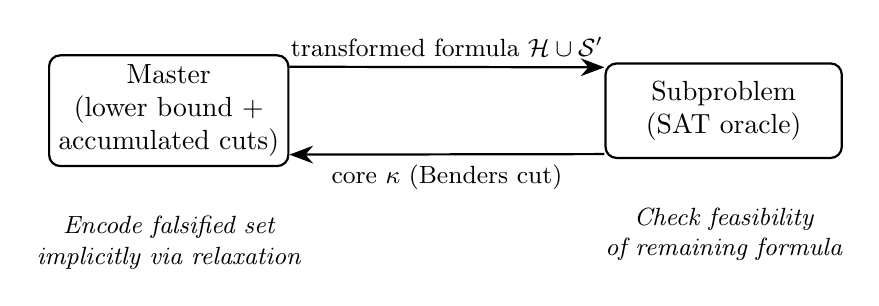
\begin{tikzpicture}[
    node distance=2.5cm and 4cm,
    block/.style={draw, rounded corners, minimum width=3cm, minimum height=1.2cm, align=center, thick},
    arrow/.style={-{Stealth[length=3mm]}, thick},
]
    \node[block] (master) {Master\\(lower bound +\\accumulated cuts)};
    \node[block, right=of master] (sub) {Subproblem\\(SAT oracle)};

    \draw[arrow] (master.20) -- node[above,font=\small] {transformed formula $\mathcal{H} \cup \mathcal{S}'$} (sub.160);
    \draw[arrow] (sub.200) -- node[below,font=\small] {core $\kappa$ (Benders cut)} (master.340);

    \node[below=0.5cm of master,font=\small\itshape,align=center] {Encode falsified set\\implicitly via relaxation};
    \node[below=0.5cm of sub,font=\small\itshape,align=center] {Check feasibility\\of remaining formula};
\end{tikzpicture}
\caption{Core-guided MaxSAT as Logic-Based Benders Decomposition. The SAT oracle acts as the subproblem; each unsatisfiable core yields a combinatorial Benders cut.}
\label{fig:benders}
\end{figure}

%----------------------------------------------------------------------
\section{IHS MaxSAT as Dantzig--Wolfe Decomposition}
\label{sec:dw}
%----------------------------------------------------------------------

\subsection{The Implicit Hitting Set Framework}

The IHS algorithm~\citep{davies2011solving,moreno2013implicit} operates as follows:
\begin{enumerate}
\item \textbf{Master problem (IP solver):} Compute a minimum-cost hitting set $H^*$ of all cores found so far. That is, solve
\[
\min \sum_{i=1}^{m} w(s_i)\, y_i \quad \text{s.t.} \quad \sum_{s_i \in \kappa_j} y_i \geq 1 \;\; \forall j = 1,\ldots,k, \quad y_i \in \{0,1\}.
\]
\item \textbf{Oracle (SAT solver):} Check whether removing the clauses in $H^*$ from $\mathcal{S}$ makes the formula satisfiable. If yes, $H^*$ is optimal; stop. If not, the SAT solver returns a new core $\kappa_{k+1}$ that is not hit by $H^*$.
\item Add $\kappa_{k+1}$ as a new constraint and repeat.
\end{enumerate}

\subsection{The Dantzig--Wolfe Connection via LP Duality}

To see the Dantzig--Wolfe structure, consider the LP dual of the hitting set
formulation~\eqref{eq:maxsat-obj}--\eqref{eq:maxsat-core}. Let $\mathcal{K} =
\{\kappa_1, \ldots, \kappa_N\}$ be the set of all cores, and let $\lambda_j
\geq 0$ be the dual variable for core $\kappa_j$. The dual LP is:
\begin{align}
\max \quad & \sum_{j=1}^{N} \lambda_j \label{eq:dual-obj}\\
\text{s.t.} \quad & \sum_{j \,:\, s_i \in \kappa_j} \lambda_j \leq w(s_i) \quad \forall i = 1,\ldots,m, \label{eq:dual-pack}\\
& \lambda_j \geq 0. \label{eq:dual-nn}
\end{align}
This is a \emph{packing} problem over cores: find a maximum-weight fractional
packing of cores subject to the capacity of each soft clause.

Since the number of cores~$N$ is exponential, this dual cannot be solved
directly. However, it has the structure required for \emph{column generation}
(the algorithmic engine of Dantzig--Wolfe decomposition):
\begin{itemize}
\item The \textbf{restricted master} is the dual LP~\eqref{eq:dual-obj}--\eqref{eq:dual-nn} restricted to the cores $\kappa_1, \ldots, \kappa_k$ discovered so far. Each core $\kappa_j$ corresponds to a \emph{column} (variable $\lambda_j$) in this dual.
\item The \textbf{pricing subproblem} asks: does there exist a core $\kappa$ not in the current restricted master that has positive reduced cost? In the dual~\eqref{eq:dual-obj}--\eqref{eq:dual-nn}, this amounts to finding a core $\kappa$ such that $\mathcal{H} \cup \kappa$ is unsatisfiable and $\kappa$ is not hit by the current primal solution. The SAT oracle answers exactly this question.
\end{itemize}

\begin{center}
\begin{tabular}{lll}
\toprule
\textbf{Dantzig--Wolfe component} & \textbf{IHS MaxSAT analog} \\
\midrule
Restricted master (dual) & Packing LP over known cores \\
Column & Core $\kappa_j$ (dual variable $\lambda_j$) \\
Pricing subproblem & SAT oracle: find unhit core \\
Negative reduced cost & Core not hit by current hitting set \\
\midrule
Restricted master (primal) & Hitting set IP over known cores \\
New constraint (row) & New core $\kappa_{k+1}$ \\
\bottomrule
\end{tabular}
\end{center}

\begin{proposition}
The IHS algorithm is a primal-side implementation of column generation on
the dual of the MaxSAT hitting set LP. Each new core discovered by the SAT
oracle acts simultaneously as:
\begin{enumerate}
\item a new \emph{row} (constraint) in the primal hitting set master, and
\item a new \emph{column} (variable) in the dual packing master.
\end{enumerate}
By LP duality, adding a row to the primal is equivalent to adding a column to
the dual. Hence the IHS algorithm is a Dantzig--Wolfe procedure on the dual
formulation.
\end{proposition}

\begin{figure}[t]
\centering
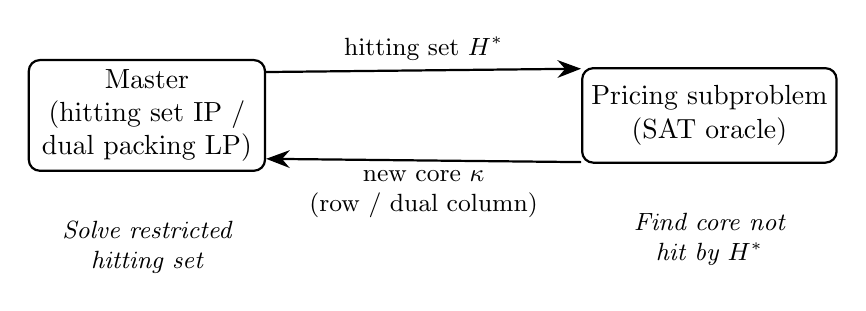
\begin{tikzpicture}[
    node distance=2.5cm and 4cm,
    block/.style={draw, rounded corners, minimum width=3cm, minimum height=1.2cm, align=center, thick},
    arrow/.style={-{Stealth[length=3mm]}, thick},
]
    \node[block] (master) {Master\\(hitting set IP /\\dual packing LP)};
    \node[block, right=of master] (sub) {Pricing subproblem\\(SAT oracle)};

    \draw[arrow] (master.20) -- node[above,font=\small] {hitting set $H^*$} (sub.160);
    \draw[arrow] (sub.200) -- node[below,font=\small,align=center] {new core $\kappa$\\(row / dual column)} (master.340);

    \node[below=0.5cm of master,font=\small\itshape,align=center] {Solve restricted\\hitting set};
    \node[below=0.5cm of sub,font=\small\itshape,align=center] {Find core not\\hit by $H^*$};
\end{tikzpicture}
\caption{IHS MaxSAT as Dantzig--Wolfe Decomposition (dual view). The SAT oracle acts as the pricing subproblem; each new core is a column in the dual packing LP.}
\label{fig:dw}
\end{figure}

\subsection{LP Bounds and Convergence}

In Dantzig--Wolfe decomposition, the restricted master LP provides a bound
that improves monotonically as columns are added, converging to the LP
optimum. Similarly, in IHS, adding more cores tightens the LP relaxation of
the hitting set master. \citet{davies2013exploiting} showed that solving the
hitting set master as an IP (rather than an LP) accelerates convergence
in practice by providing both primal feasible solutions and dual bounds
simultaneously.

The work of \citet{katsirelos2023analysis} further showed that core-guided
algorithms such as OLL implicitly compute feasible dual solutions of an LP
that encodes the same hitting set structure. This means that both families
of algorithms---core-guided and IHS---are optimizing over the \emph{same}
LP relaxation, but from opposite sides of duality.

\subsection{What the Analogy Preserves, and What It Doesn't}
\label{sec:preserves}

The Dantzig--Wolfe view is illuminating but is not a textbook instantiation
of column generation. To use it responsibly, it helps to be explicit about
which structural features carry over and which do not.

\paragraph{What the analogy preserves.} The most robust part of the analogy
is the \emph{row--column duality between cuts and cores}. Adding a hitting-set
row $\sum_{s_i \in \kappa} y_i \geq 1$ to the primal IP
formulation~\eqref{eq:maxsat-obj}--\eqref{eq:maxsat-int} is exactly equivalent,
by LP duality, to introducing a new variable~$\lambda_\kappa$ in the dual
packing LP~\eqref{eq:dual-obj}--\eqref{eq:dual-nn}. This is the same
row-to-column transformation that mediates the Benders/Dantzig--Wolfe duality
in classical OR. Likewise, the \emph{reduced-cost interpretation of an unhit
core} is exact: given the current dual prices~$\bar{y}$ (a fractional hitting
set from the LP relaxation of the master), a core $\kappa$ has positive
reduced cost in the dual packing problem iff
$\sum_{s_i \in \kappa} \bar{y}_i < 1$, which is precisely the condition that
$\kappa$ is not (fractionally) hit. The SAT oracle is therefore a sound
implementation of pricing: if it finds a new core, the master's LP bound is
not yet optimal; if it cannot, the master's solution is LP-optimal.

\paragraph{What the analogy does not preserve.} Three classical features of
Dantzig--Wolfe break down here, and recognizing this prevents over-claiming.

\begin{enumerate}
\item \textbf{Pricing is NP-complete, not polynomial.} In textbook
Dantzig--Wolfe the subproblem is a tractable LP with block structure (network
flow, knapsack, etc.) and pricing returns a column in polynomial time. Here
pricing is a SAT call---NP-complete in general. The high per-iteration cost
is real, and many of the convergence-rate analyses for column generation (e.g.,
worst-case iteration bounds in terms of LP geometry) do not transfer directly.
What does transfer is that pricing returns a column with negative reduced cost
\emph{when one exists}; modern SAT solvers are sound and complete oracles,
which is what the analogy actually requires.
\item \textbf{The master is solved as an IP, not an LP.} Practical IHS solves
the master as an integer program to obtain feasible hitting sets directly
(\citealp{davies2013exploiting}), which is non-standard for column generation
and closer to branch-and-price without the branching. In particular, the
\emph{LP relaxation of the master is not what is solved at each iteration},
so the dual bound used by classical pricing arguments is not directly
available. The analogy holds at the level of the underlying LP, but the
implementation departs from it.
\item \textbf{Columns are generated, not enumerated convex combinations.}
Standard Dantzig--Wolfe represents the subproblem polytope $\mathcal{P}$ via
its extreme points, with the master expressing $x$ as a convex combination
$x = \sum_k \lambda_k p^k$. In MaxSAT there is no such polytope to
parameterize; cores are constraints rather than points, and the columns
$\lambda_\kappa$ live only in the \emph{dual}. Equivalently: the
MaxSAT version of Dantzig--Wolfe is column generation on the
\emph{constraint-generation dual} of an exponentially-constrained covering
problem, not on a Minkowski decomposition of a primal polytope. This is a
known but more specialized setting in OR (sometimes called ``constraint
generation viewed dually as column generation''), and it is the version
that fits MaxSAT.
\end{enumerate}

\paragraph{Net assessment.} The analogy is sound at the level of LP duality
between primal cuts and dual columns, and at the level of the pricing oracle's
specification. It is loose at the level of complexity, convergence rates, and
master tractability. The useful consequence is that techniques whose
correctness depends only on the row--column duality---in-out separation,
dual stabilization, Lagrangian smoothing of master prices---should transfer.
Techniques that rely on polynomial pricing or LP master geometry should not
be expected to transfer without adaptation.

%----------------------------------------------------------------------
\section{A Worked Example}
\label{sec:example}
%----------------------------------------------------------------------

To make the row--column duality concrete, we trace both algorithms on the
same small instance and compare what each one accumulates.

\paragraph{Instance.} No hard clauses; four unit soft clauses, all of
weight~1:
\[
  s_1 = a,\quad s_2 = \neg a,\quad s_3 = b,\quad s_4 = \neg b.
\]
The optimum is $\mathit{OPT} = 2$: any solution must falsify exactly one of
$\{s_1, s_2\}$ and one of $\{s_3, s_4\}$. The only minimal cores are
$\kappa_1 = \{s_1, s_2\}$ and $\kappa_2 = \{s_3, s_4\}$.

\paragraph{Hitting-set LP.} The MaxSAT IP and its LP relaxation are
\[
  \min\; y_1+y_2+y_3+y_4
  \;\;\text{s.t.}\;\; y_1+y_2 \geq 1,\;\; y_3+y_4 \geq 1,\;\; y \in [0,1]^4,
\]
with LP value~$2$ (integrality gap zero, since this matrix is balanced). The
dual packing LP is
\[
  \max\; \lambda_1 + \lambda_2
  \;\;\text{s.t.}\;\; \lambda_1 \leq w(s_1),\, \lambda_1 \leq w(s_2),\,
  \lambda_2 \leq w(s_3),\, \lambda_2 \leq w(s_4),\, \lambda \geq 0,
\]
with optimum $\lambda_1 = \lambda_2 = 1$, value~$2$.

\paragraph{Trace of core-guided (Algorithm~\ref{alg:cg}).}
\begin{enumerate}
\item $\textsc{SAT}(\mathcal{H} \cup \mathcal{S}')$ on the four units:
\textbf{UNSAT}. Return core $\kappa_1 = \{s_1, s_2\}$. Set
$\delta = 1$, $\mathit{lb} = 1$. \textsc{Relax} weakens
$s_1 \mapsto a \vee r_1$ and $s_2 \mapsto \neg a \vee r_2$ and adds the soft
cardinality constraint $r_1 + r_2 \geq 1$ (weight~1).
\item $\textsc{SAT}$ on the relaxed formula: \textbf{UNSAT}. The new core
is $\kappa_2 = \{s_3, s_4\}$. Set $\delta = 1$, $\mathit{lb} = 2$. Relax
$s_3, s_4$ analogously, adding $r_3 + r_4 \geq 1$.
\item $\textsc{SAT}$: \textbf{SAT}. Set, e.g., $a = \mathit{true}$,
$b = \mathit{true}$, $r_2 = r_4 = 1$, $r_1 = r_3 = 0$. Return cost
$\mathit{lb} = 2$.
\end{enumerate}

\paragraph{Trace of IHS (Algorithm~\ref{alg:ihs}).}
\begin{enumerate}
\item $\mathcal{K} = \emptyset$. The IP master is unconstrained, so $H^* =
\emptyset$. $\textsc{SAT}$ on the full formula: \textbf{UNSAT}, core
$\kappa_1 = \{s_1, s_2\}$.
\item $\mathcal{K} = \{\kappa_1\}$. The IP master $\min\sum y_i$ s.t.\
$y_1 + y_2 \geq 1$ gives, e.g., $H^* = \{s_1\}$ (cost~1). $\textsc{SAT}$ on
$\{s_2, s_3, s_4\}$: \textbf{UNSAT}, core $\kappa_2 = \{s_3, s_4\}$.
\item $\mathcal{K} = \{\kappa_1, \kappa_2\}$. The IP master gives, e.g.,
$H^* = \{s_1, s_3\}$ (cost~2). $\textsc{SAT}$ on $\{s_2, s_4\}$ = $\neg a
\wedge \neg b$: \textbf{SAT}. Return cost~$2$.
\end{enumerate}

\paragraph{Side-by-side comparison.} Both algorithms discover exactly the
same two cores $\{\kappa_1, \kappa_2\}$, in the same order, and terminate with
the same optimum. What differs is the data structure that accumulates them
(Table~\ref{tab:trace}):

\begin{table}[h]
\centering
\caption{The two algorithms accumulate the same information in dual forms.}
\label{tab:trace}
\begin{tabular}{lll}
\toprule
\textbf{Iteration} & \textbf{Core-guided accumulates} & \textbf{IHS accumulates} \\
\midrule
1 ($\kappa_1$ found) & relaxation vars $r_1, r_2$;     & primal row $y_1 + y_2 \geq 1$;     \\
                     & cardinality $r_1 + r_2 \geq 1$  & dual column $\lambda_1$            \\
2 ($\kappa_2$ found) & relaxation vars $r_3, r_4$;     & primal row $y_3 + y_4 \geq 1$;     \\
                     & cardinality $r_3 + r_4 \geq 1$  & dual column $\lambda_2$            \\
\midrule
After 2 iter.\ & $\mathit{lb} = 2$ encoded by         & $H^* \in \{ \{s_1,s_3\}, \{s_1,s_4\}, \{s_2,s_3\}, \{s_2,s_4\} \}$, \\
               & relaxation structure                  & all of cost~2 \\
\bottomrule
\end{tabular}
\end{table}

The two cardinality constraints accumulated on the core-guided side are
exactly the two hitting-set rows on the IHS side---syntactically rewritten on
the relaxation variables rather than the original $y_i$, but encoding the
same information. By LP duality, those two rows correspond to two dual
columns $\lambda_1, \lambda_2$ in the packing LP. After two iterations both
sides have identified the LP optimum~$\lambda_1 = \lambda_2 = 1 = \mathit{OPT}$,
one by raising $\mathit{lb}$ through formula transformations (Benders-style),
the other by computing it explicitly via an IP master (Dantzig--Wolfe-style on
the dual).

%----------------------------------------------------------------------
\section{The Unified Picture}
\label{sec:unified}
%----------------------------------------------------------------------

The preceding analysis reveals a clean duality diagram connecting the four
methods:

\begin{figure}[h]
\centering
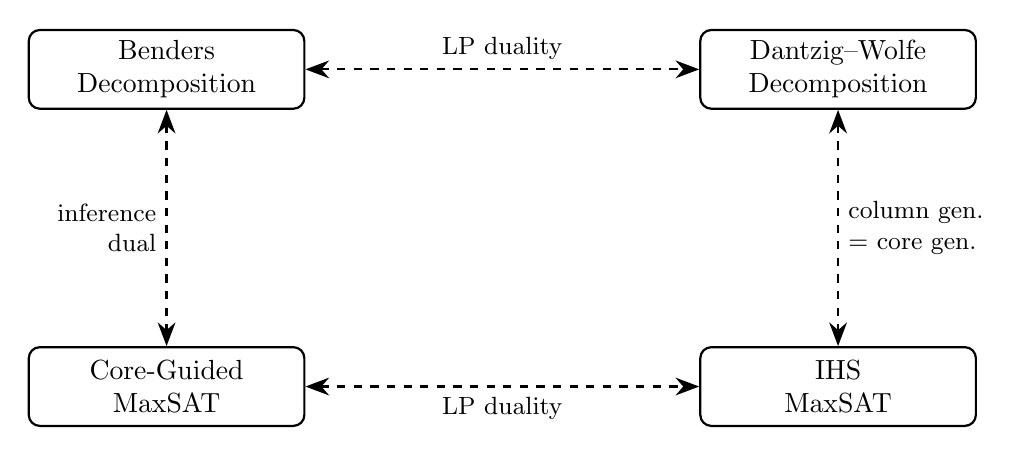
\begin{tikzpicture}[
    node distance=3cm and 5cm,
    block/.style={draw, rounded corners, minimum width=3.5cm, minimum height=1cm, align=center, thick},
    arrow/.style={{Stealth[length=3mm]}-{Stealth[length=3mm]}, thick, dashed},
]
    \node[block] (benders) {Benders\\Decomposition};
    \node[block, right=of benders] (dw) {Dantzig--Wolfe\\Decomposition};
    \node[block, below=of benders] (cg) {Core-Guided\\MaxSAT};
    \node[block, below=of dw] (ihs) {IHS\\MaxSAT};

    \draw[arrow] (benders) -- node[above,font=\small] {LP duality} (dw);
    \draw[arrow] (cg) -- node[below,font=\small] {LP duality} (ihs);
    \draw[arrow] (benders) -- node[left,font=\small,align=right] {inference\\dual} (cg);
    \draw[arrow] (dw) -- node[right,font=\small,align=left] {column gen.\\= core gen.} (ihs);
\end{tikzpicture}
\caption{The duality square connecting decomposition methods and MaxSAT algorithms.}
\label{fig:square}
\end{figure}

\begin{itemize}
\item \textbf{Horizontal axis (LP duality):} Benders and Dantzig--Wolfe are
dual to each other; core-guided and IHS are dual to each other in the same
sense. Adding a cut in one is adding a column in the other.
\item \textbf{Vertical axis (generalization):} Core-guided MaxSAT is an
instance of LBBD where the inference dual replaces the LP dual. IHS MaxSAT
is an instance of Dantzig--Wolfe where the pricing oracle is a SAT solver
rather than an LP.
\end{itemize}

This diagram also explains empirically observed complementarities. IHS solvers
(like Dantzig--Wolfe) tend to produce good primal solutions quickly because
the master IP yields feasible hitting sets at each iteration. Core-guided
solvers (like Benders) tend to produce strong dual bounds because each core
directly tightens the relaxation. This mirrors the well-known tradeoff in
OR between cut-based and column-based approaches.

%----------------------------------------------------------------------
\section{Transferable Techniques from OR to MaxSAT}
\label{sec:techniques}
%----------------------------------------------------------------------

Section~\ref{sec:preserves} identified exactly which structural features carry
over from Dantzig--Wolfe and Benders to the MaxSAT setting. The useful
consequence is that techniques whose correctness depends only on row--column
duality and the soundness of the pricing oracle should transfer essentially
unchanged. This section collects the most actionable candidates, in roughly
increasing order of implementation cost.

\subsection{Cross-Family Warm-Starting}

The cheapest hybrid technique is initialization. A short run of one algorithm
produces information that warm-starts the other, just as OR practitioners
routinely warm-start Benders or Dantzig--Wolfe masters with cuts or columns
from a heuristic phase.

\begin{itemize}
\item \emph{IHS seeded by core-guided.} Run Algorithm~\ref{alg:cg} for a fixed
iteration budget; harvest all cores it has discovered (whether explicitly
extracted or implicit in the relaxation structure). Initialize
Algorithm~\ref{alg:ihs} with $\mathcal{K}$ set to this collection. The first
IP master solve already returns a non-trivial $H^*$, skipping the cold-start
phase where IHS has no master structure to exploit.
\item \emph{Core-guided seeded by IHS or MCS enumeration.} Conversely, a quick
enumeration of minimal correction sets~\citep{liffiton2008algorithms} yields
cores by hitting-set duality. Pre-relaxing the formula along these cores gives
Algorithm~\ref{alg:cg} a head start on the lower bound.
\end{itemize}

This requires no algorithmic surgery---only sharing the data structure that
holds discovered cores---and so is the most accessible of the techniques
listed.

\subsection{Pareto-Optimal Core Selection}

A SAT oracle that returns UNSAT typically admits many valid cores; modern
conflict-driven solvers return one based on internal heuristics, not on what
is most useful to the master. The Benders literature provides a principled
answer: \citet{magnanti1981accelerating} select, among multiple valid cuts,
the one that is \emph{non-dominated} (Pareto-optimal) with respect to a
reference interior point of the master's feasible region.

The MaxSAT analog is concrete. Given an UNSAT call and a current fractional
hitting set~$\bar{y}$ (the LP relaxation of the master), prefer cores
$\kappa$ that maximize the violation $1 - \sum_{s_i \in \kappa} \bar{y}_i$.
Among cores with the same violation, prefer those that are minimal. This
couples MUS extraction with the master's current state, replacing the SAT
solver's internal heuristic with a Magnanti--Wong-style criterion. Because
soundness does not depend on which specific core is returned, this is a pure
orthogonal improvement and can be layered on top of existing IHS or
core-guided implementations.

\subsection{Dual Stabilization for IHS}

The IHS master, viewed as the dual of the packing
LP~\eqref{eq:dual-obj}--\eqref{eq:dual-nn}, suffers from the same instabilities
that plague column generation: degenerate dual solutions cause $H^*$ to
oscillate between alternative optima, slowing convergence in the late phase
(``tailing off''). Three OR techniques address this directly.

\paragraph{Wentges-style box stabilization.}
\citet{wentges1997weighted} adds a penalty term to the master that discourages
dual prices from drifting too far from a current \emph{stability center}.
Translated to IHS: maintain a reference fractional hitting set~$\bar{y}$ and
replace the master objective $\sum_i w(s_i)\, y_i$ by
$\sum_i w(s_i)\, y_i + \alpha \|y - \bar{y}\|_1$ for a decaying
penalty~$\alpha$. The stability center is updated when the SAT oracle
confirms progress. Implementation cost is low (one additional term in the IP
master), and correctness is preserved because $\alpha \to 0$ at termination.

\paragraph{In-out separation.}
\citet{benameur2007stabilization} interpolate between the current dual
solution and an interior point of the feasible dual region before pricing.
The MaxSAT analog: instead of calling the SAT oracle on $\mathcal{S}
\setminus H^*$, call it on $\mathcal{S} \setminus H^{\mathrm{io}}$, where
$H^{\mathrm{io}}$ is a convex combination of $H^*$ with a known feasible
(possibly suboptimal) hitting set. Cores extracted from interior points
tend to be deeper---they hit more constraints simultaneously---and they
damp master oscillation.

\paragraph{Bundle / proximal methods.}
For large-scale instances, bundle methods maintain a polyhedral approximation
of the dual function with proximal regularization. They could be adapted to
IHS by keeping a small set of past hitting sets and choosing the next probe
via a proximal step; this is more disruptive to implement but is the standard
heavy-machinery response to tailing-off in column generation.

\subsection{Price-Aware Core Extraction}

A more invasive idea draws on Lagrangian relaxation. The dual prices~$\bar{y}$
from the master's LP relaxation can be interpreted as a measure of how
``expensive'' each soft clause is to falsify. Cores composed of high-price
soft clauses contribute more to tightening the bound (a higher minimum
weight~$\delta$ in Algorithm~\ref{alg:cg}; a tighter packing constraint in
the dual~\eqref{eq:dual-pack}). One can therefore bias the SAT oracle's
search toward such cores---e.g., by reweighting VSIDS scores by current dual
prices, or by augmenting branching heuristics with the master's dual
information.

This is the most speculative of the techniques listed: it requires
SAT-solver modification, not just outer-loop changes. But it has a clean
theoretical foundation: it is the MaxSAT analog of running the pricing
subproblem with the current dual prices as objective, which is the defining
operation of column generation.

\subsection{Toward Hybrid Primal--Dual Solvers}

Together, the techniques above point toward a unified solver that maintains
both representations simultaneously: an explicit IP master (IHS-side) and a
transformed working formula (core-guided side). At each iteration, the
algorithm chooses whether the next core should be extracted by an IHS-style
probe (using $H^*$ as assumptions) or by a core-guided probe (on the current
relaxed formula), based on which is more likely to produce a useful cut. The
LP-based reformulation of OLL by~\citet{katsirelos2025core} provides a
natural starting point, since it makes the dual computations underlying
core-guided algorithms explicit and therefore composable with an IHS-style
IP master.

%----------------------------------------------------------------------
\section{Discussion}
\label{sec:discussion}
%----------------------------------------------------------------------

\paragraph{Implications for algorithm design.}
The decomposition viewpoint suggests a portfolio of techniques transferable
from OR to MaxSAT; these are developed in Section~\ref{sec:techniques}, from
the most readily deployable (cross-family warm-starting) to the most
speculative (price-aware core extraction inside the SAT solver).

\paragraph{Limitations.}
The analogy is structural, not exact. Section~\ref{sec:preserves} gives the
detailed breakdown of what is preserved (row--column duality between cuts and
cores; soundness of the SAT oracle as a pricing routine) and what is not
(polynomial pricing, LP master geometry, primal Minkowski decomposition).

%----------------------------------------------------------------------
\section{Future Work}
\label{sec:future}
%----------------------------------------------------------------------

The viewpoint developed here makes several concrete predictions and surfaces
open questions worth pursuing.

\paragraph{Empirical validation of transferred techniques.} The techniques
collected in Section~\ref{sec:techniques} are presented on theoretical
grounds. Each one yields a falsifiable empirical claim: cross-family
warm-starting should reduce IHS cold-start iterations on benchmark families
where core-guided is known to find good lower bounds quickly; Wentges-style
stabilization should reduce the tailing-off plateau in IHS solve time on
instances with degenerate hitting-set LPs; Pareto-optimal core selection
should reduce iteration counts on instances with many redundant cores.
Systematic experimental study of these predictions---ideally on the MSE
benchmarks---would be the most direct way to validate (or refute) the
operational value of the analogy. We are not aware of any such study to date.

\paragraph{The weighted case.} The cleanest LP encodings of core-guided
algorithms~\citep{katsirelos2023analysis} are for unweighted instances. The
weighted case is where most practical interest lies, and where the
bound-tightening story is more delicate: weight-stratified core extraction,
weight splitting, and the interaction with $\delta$ in
Algorithm~\ref{alg:cg} change the structure of the implicit master in ways
that the unweighted analysis does not directly cover. Establishing whether the
Dantzig--Wolfe analogy is exact in the weighted case, or merely heuristic, is
an open question.

\paragraph{Filling in the square.} Figure~\ref{fig:square} has four corners,
but OR offers richer machinery built on top of each: \emph{branch-and-price}
extends Dantzig--Wolfe with branching on master variables; \emph{Benders
branch-and-cut} interleaves cut generation with branching in a single
search tree. The MaxSAT analogs of these are largely missing from the
landscape. IHS with branching on hitting-set decisions is one natural
direction; core-guided algorithms equipped with an explicit IP master in the
spirit of~\citet{davies2013exploiting} are arguably a partial Benders
branch-and-cut. Naming the empty cells of the analogy is often where the
genuine research opportunities lie.

%----------------------------------------------------------------------
\section{Part I Conclusion}
\label{sec:conclusion}
%----------------------------------------------------------------------

We have presented explicit structural correspondences between two families of
MaxSAT algorithms and two classical decomposition methods from operations
research. Core-guided MaxSAT algorithms implement a form of Logic-Based
Benders Decomposition, where unsatisfiable cores serve as combinatorial
Benders cuts derived through inference duality. Implicit Hitting Set
algorithms implement a form of Dantzig--Wolfe decomposition (viewed through LP
duality), where the SAT oracle acts as a pricing subproblem generating new
columns in the dual packing formulation. These connections are mediated by LP
duality: the hitting set (primal) and core packing (dual) formulations of
MaxSAT stand in the same relationship as Benders and Dantzig--Wolfe masters.

Making these connections explicit opens a two-way transfer of techniques
between the OR and SAT communities, from cut strengthening and stabilization
to hybrid primal-dual algorithms that leverage the strengths of both
decomposition paradigms.




%======================================================================
\section{Is IHS for MaxSAT Equivalent to Dantzig--Wolfe? A Worked Example and a Counterexample}
\label{sec:part2}
%======================================================================

%----------------------------------------------------------------------
\subsection{The Claim, Stated Precisely}
\label{sec:claim}
%----------------------------------------------------------------------

\cref{sec:part1} argued that Implicit Hitting Set (IHS) MaxSAT solvers
implement Dantzig--Wolfe (DW) decomposition, viewed through LP duality. Here we
test that claim concretely. We first state the equivalence precisely and prove
the row/column duality that underlies it. We then work a small instance step by
step, running IHS and DW column generation side by side and observing that they
generate the same cores, in the same order, with the same bounds, and terminate
with the same value. Finally we exhibit a counterexample: a three-clause
instance on which DW column generation terminates at the value $3/2$ while
IHS---and the true MaxSAT optimum---is $2$. The resolution is sharp: \textbf{IHS
with an LP master is exactly DW on the dual core-packing LP, but the IHS used in
practice solves the master as an integer program, which is strictly stronger than
DW and breaks literal equivalence.} The equivalence is therefore real but
conditional, and the condition (LP vs.\ integer master) is exactly the
integrality gap of the hitting-set polytope.

Fix a weighted partial MaxSAT instance $\langle \mathcal{H}, \mathcal{S}, w
\rangle$ with soft clauses $\mathcal{S} = \{s_1,\dots,s_m\}$ and weights
$w_i = w(s_i) > 0$. For $y \in \{0,1\}^m$ read $y_i = 1$ as ``$s_i$ is
falsified.'' Let $\mathcal{K}$ be the (exponential) family of all cores
$\kappa \subseteq \mathcal{S}$, i.e.\ subsets with $\mathcal{H} \cup \kappa$
unsatisfiable. MaxSAT is the \emph{minimum-cost hitting set} over $\mathcal{K}$:
\begin{align}
(\mathrm{IP})\qquad
z^\star = \min \;\; & \textstyle\sum_{i} w_i\, y_i \notag\\
\text{s.t.} \;\; & \textstyle\sum_{s_i \in \kappa} y_i \ge 1 \quad \forall \kappa \in \mathcal{K}, \label{eq:hit}\\
& y_i \in \{0,1\}. \notag
\end{align}
Its LP relaxation replaces $y_i \in \{0,1\}$ by $y_i \ge 0$ (the upper bound
$y_i \le 1$ is slack at the optimum of a minimization). Call its value
$z^\star_{\mathrm{LP}}$. The LP \emph{dual} assigns a variable
$\lambda_\kappa \ge 0$ to each core and is a \emph{fractional core packing}:
\begin{align}
(\mathrm{D})\qquad
z^\star_{\mathrm{LP}} = \max \;\; & \textstyle\sum_{\kappa} \lambda_\kappa \notag\\
\text{s.t.} \;\; & \textstyle\sum_{\kappa \ni s_i} \lambda_\kappa \le w_i \quad \forall i = 1,\dots,m, \label{eq:pack}\\
& \lambda_\kappa \ge 0. \notag
\end{align}

\paragraph{What ``Dantzig--Wolfe'' means here.} Dantzig--Wolfe decomposition
reformulates a structured LP so that its variables are indexed by an exponential
family (the extreme points of a subproblem polyhedron), and solves the
reformulation by \emph{column generation}: maintain a \emph{restricted master}
with only a working subset of columns, read off dual prices, and call a
\emph{pricing subproblem} that either returns a new column of negative reduced
cost or certifies optimality. We take ``IHS is DW'' to mean precisely:
\emph{IHS is column generation applied to the dual packing LP}~\eqref{eq:pack},
where each core is a column.

\paragraph{What IHS does.} IHS keeps a working set $\mathcal{K}_t \subseteq
\mathcal{K}$ of \emph{discovered} cores, solves the \emph{restricted} master
\eqref{eq:hit} over $\mathcal{K}_t$ to get $H_t^\star$ (the set of $s_i$ with
$y_i = 1$), then calls a SAT oracle on $\mathcal{H} \cup (\mathcal{S} \setminus
H_t^\star)$. If SAT, $H_t^\star$ is an achievable correction set and, being a
minimum hitting set of all known cores, is optimal: stop. If UNSAT, the oracle
returns a core $\kappa$ \emph{not hit} by $H_t^\star$; add it and repeat. The
only design choice we vary below is whether the master \eqref{eq:hit} is solved
as an integer program (\textbf{IHS-IP}, the practical solver, e.g.\ MaxHS) or as
its LP relaxation (\textbf{IHS-LP}).

%----------------------------------------------------------------------
\subsection{The Exact Equivalence (LP Master)}
\label{sec:equiv}
%----------------------------------------------------------------------

The bridge is the textbook fact that \emph{generating rows of an LP is
generating columns of its dual}. We state it for our setting.

\begin{lemma}[Row generation $=$ column generation across duality]
\label[lemma]{lem:rowcol}
Let $\mathcal{K}_t \subseteq \mathcal{K}$. The restricted primal LP---
\eqref{eq:hit} relaxed to $y\ge0$ and limited to cores in $\mathcal{K}_t$---and
the restricted dual---\eqref{eq:pack} limited to the columns $\{\lambda_\kappa :
\kappa \in \mathcal{K}_t\}$---are an LP dual pair. Consequently:
\begin{enumerate}
\item[(i)] they have equal optimal value $v_t$, and the primal optimum $y^{(t)}$
is the vector of dual prices of the restricted dual;
\item[(ii)] a core $\kappa \in \mathcal{K}\setminus\mathcal{K}_t$ is
\emph{violated} by $y^{(t)}$ in the primal, i.e.\ $\sum_{s_i \in \kappa}
y^{(t)}_i < 1$, \emph{iff} the column $\lambda_\kappa$ has \emph{strictly
positive reduced cost} $\bar c_\kappa = 1 - \sum_{s_i\in\kappa} y^{(t)}_i$ in
the dual;
\item[(iii)] adding $\kappa$ to $\mathcal{K}_t$ adds one row to the primal and,
identically, one column to the dual.
\end{enumerate}
\end{lemma}

\begin{proof}
The dual of $\min\{w^\top y : A_t y \ge \mathbf 1,\ y \ge 0\}$ is $\max\{\mathbf
1^\top\lambda : A_t^\top \lambda \le w,\ \lambda \ge 0\}$, where $A_t$ is the
core-incidence matrix whose rows are the cores in $\mathcal{K}_t$. The first is
the restricted primal, the second the restricted dual; (i) is strong LP duality
and complementary reading of the simplex multipliers. For (ii), the dual
objective coefficient of $\lambda_\kappa$ is $1$ and its column in $A_t^\top$ is
the incidence vector of $\kappa$. Since the dual is a \emph{maximization}, we
adopt the standard convention that an entering column is one with
\emph{strictly positive} reduced cost (objective coefficient minus the
dual-price contribution). With prices $y^{(t)}$ the reduced cost is
$\bar c_\kappa = 1 - \sum_{s_i \in \kappa} y^{(t)}_i$, positive exactly when
$\kappa$ is under-hit. (iii) is immediate from the transpose relationship.
\end{proof}

\begin{proposition}[IHS-LP is Dantzig--Wolfe on the dual]
\label[proposition]{prop:equiv}
Run IHS-LP and column generation on the dual packing
LP~\eqref{eq:pack} from the same initial working set, with the SAT oracle as the
pricing routine, and assume:
\begin{itemize}
\item[(a)] both runs use a \emph{deterministic} LP solver that, on inputs with
the same constraint matrix, returns the same basic optimum (so degeneracy is
broken identically on both sides); and
\item[(b)] a common tie-breaking rule selects, among multiple violated /
under-priced cores, the one the oracle returns.
\end{itemize}
Then at every iteration the two algorithms hold the same working set
$\mathcal{K}_t$, the same master value $v_t$, and---given (b)---generate the
\emph{same} core. Both terminate with value $z^\star_{\mathrm{LP}}$.
\end{proposition}

\begin{proof}
Induction on $t$. The master values agree by \cref{lem:rowcol}(i). At the
pricing step, IHS-LP seeks a core violated by $y^{(t)}$; column generation seeks
a column of positive reduced cost; by \cref{lem:rowcol}(ii) these are the
\emph{same set of candidate cores}, so under (b) a shared oracle returns the
same $\kappa$, and by (iii) the two working sets stay equal. Termination is
simultaneous: ``no violated core'' $=$ ``no positive-reduced-cost column,'' and
the common value is the full LP optimum $z^\star_{\mathrm{LP}}$ because all
violated cores have been priced out.
\end{proof}

\begin{remark}[Degeneracy]
\label[remark]{rem:degeneracy}
Hypothesis (a) is genuinely needed: the restricted LP can have multiple optima
(e.g.\ on $K_3$ (\cref{sec:counter}) after the single core $\kappa_{12}$, both
$y=(1,0,0)$ and $y=(0,1,0)$ are optimal; after a second core the optimum
becomes unique again---the clause shared by the two cores),
and two solvers returning different bases will ask the SAT oracle different
pricing questions and may extract different cores. The master \emph{value}
still agrees in lockstep---only the trajectory of generated cores can fork.
This is the same degeneracy that motivates dual-stabilization techniques
(\cref{sec:techniques}).
\end{remark}

\begin{remark}[Fractional pricing is not one SAT call]
\label[remark]{rem:fracpricing}
\Cref{prop:equiv} equips IHS-LP with an oracle that, given the
\emph{fractional} prices $y^{(t)}$, finds a core $\kappa$ with
$\sum_{s_i \in \kappa} y^{(t)}_i < 1$ or certifies that none exists. When
$y^{(t)}$ is integral, this is exactly one SAT call on
$\mathcal{H} \cup (\mathcal{S} \setminus H_t^\star)$---the standard IHS
oracle---and that is the case throughout the $P_4$ trace of
\cref{sec:worked}. For genuinely fractional $y^{(t)}$, however, separation
asks for an unsatisfiable subset of fractional weight below~$1$. This is a
\emph{weighted-MUS-type optimization} (find $\kappa$ minimizing $\sum_{s_i \in \kappa} y_i^{(t)}$)
that no single SAT call implements. Thus IHS-LP, unlike IHS-IP, is \emph{not}
implementable with the unmodified IHS oracle; this is a second, independent
sense in which practical IHS departs from textbook column generation.
Conveniently, the integer master of practical IHS guarantees integral prices,
which is precisely what lets a plain SAT call serve as the separation routine
(cf.\ \cref{sec:subtle}, point~2). \Cref{sec:cg-gap} develops outer-loop
approximations to exactly this fractional pricing problem.
\end{remark}

\cref{prop:equiv} is the precise, defensible content of the slogan
``IHS is Dantzig--Wolfe in the dual.'' Note three things it does \emph{not} say,
which we revisit in \cref{sec:subtle}: it concerns the \emph{LP} master; the
oracle is used as a \emph{separation} oracle (find \emph{some} violated core),
not a true DW pricing oracle (find the \emph{most} negative reduced cost); and
the dual~\eqref{eq:pack} has no convexity row $\sum_\kappa \lambda_\kappa = 1$,
so it is column generation in general, of which DW is the special case where
columns are extreme points of a fixed polyhedron.

%----------------------------------------------------------------------
\subsection{A Step-by-Step Example Where They Coincide}
\label{sec:worked}
%----------------------------------------------------------------------

We now make \cref{prop:equiv} concrete on an instance whose
hitting-set polytope is \emph{integral}, so IHS-IP, IHS-LP, and DW all agree.

\subsubsection{The Instance \texorpdfstring{$P_4$}{P4}}

Four soft \emph{unit} clauses with unit weight,
\[
s_1=(x_1),\quad s_2=(x_2),\quad s_3=(x_3),\quad s_4=(x_4),\qquad w_i = 1,
\]
and three hard clauses forbidding adjacent pairs from being true together,
\[
\mathcal{H} = \{(\bar x_1 \vee \bar x_2),\ (\bar x_2 \vee \bar x_3),\ (\bar x_3 \vee \bar x_4)\}.
\]
Setting $x_i$ true falsifies nothing in $\mathcal{H}$ by itself, so each
singleton soft set is satisfiable; a pair $\{s_i,s_j\}$ is unsatisfiable with
$\mathcal{H}$ \emph{iff} $\{i,j\}$ is an edge of the path $1{-}2{-}3{-}4$. One
checks that every $3$-subset of $\{1,2,3,4\}$ contains an edge, so the
\textbf{minimal cores are exactly the three edges} (see \cref{fig:p4-k3},
left):
\[
\kappa_a = \{s_1,s_2\},\qquad \kappa_b = \{s_2,s_3\},\qquad \kappa_c = \{s_3,s_4\}.
\]
Hitting all edges is the minimum \emph{vertex cover} of the path; the path is
bipartite, so by K\H{o}nig's theorem the LP relaxation is integral and
$z^\star = z^\star_{\mathrm{LP}} = 2$ (e.g.\ cover $\{s_2,s_3\}$; equivalently
the MaxSAT optimum keeps the independent set $\{x_1,x_3\}$ true and falsifies
two clauses).

\subsubsection{Running IHS-IP and DW in Lockstep}

We let the SAT oracle, when several cores are unhit, return them in the fixed
order $\kappa_a, \kappa_b, \kappa_c$ (any common rule works, fulfilling Hypothesis (b)
of \cref{prop:equiv} to ensure both algorithms trace the exact same path). \cref{tab:trace-p4}
traces both algorithms. For DW we report the dual prices $y^{(t)}$ (the
restricted-primal optimum) used by pricing, and the dual master value; for
IHS we report the integer hitting set $H_t^\star$ and the lower bound. Recall
the pricing test from \cref{lem:rowcol}(ii): a core $\kappa$ is improving
iff $\sum_{s_i\in\kappa} y^{(t)}_i < 1$.

\begin{table}[htbp]
\centering
\small
\begin{tabular}{c l l c l}
\toprule
$t$ & Working set $\mathcal{K}_t$ & IHS-IP master $H_t^\star$ (LB) & DW prices $y^{(t)}$ & Pricing $\to$ new core \\
\midrule
$1$ & $\emptyset$ & $\emptyset$ \;(LB $0$) & $(0,0,0,0)$ & $\kappa_a$: $0<1$ \;$\Rightarrow$ add $\kappa_a$\\
$2$ & $\{\kappa_a\}$ & $\{s_1\}$ \;(LB $1$) & $(1,0,0,0)$ & $\kappa_b$: $y_2{+}y_3{=}0$ \;$\Rightarrow$ add $\kappa_b$\\
$3$ & $\{\kappa_a,\kappa_b\}$ & $\{s_2\}$ \;(LB $1$) & $(0,1,0,0)$ & $\kappa_c$: $y_3{+}y_4{=}0$ \;$\Rightarrow$ add $\kappa_c$\\
$4$ & $\{\kappa_a,\kappa_b,\kappa_c\}$ & $\{s_2,s_3\}$ \;(LB $2$) & $(0,1,1,0)$ & all cores hit \;$\Rightarrow$ \textbf{stop} \\
\bottomrule
\end{tabular}
\caption{IHS-IP and DW column generation on $P_4$, in lockstep. The master
value (LB) and the dual master value coincide at every step ($0,1,1,2$); the
same cores are generated in the same order; both stop at $t=4$ with value $2$.}
\label{tab:trace-p4}
\end{table}

\paragraph{Reading the steps.}
\begin{itemize}
\item \textbf{$t=1$.} No cores known. Master is empty $\Rightarrow H^\star =
\emptyset$, prices $y=0$. The SAT oracle on $\mathcal{H}\cup\{x_1,x_2,x_3,x_4\}$
is UNSAT (all-true violates every hard clause) and returns $\kappa_a$. In DW,
$\bar c_{\kappa_a} = 1 - 0 = 1 > 0$: the identical column.
\item \textbf{$t=2$.} Master $\min \sum y_i$ s.t.\ $y_1+y_2 \ge 1$ gives
$H^\star=\{s_1\}$ and dual prices $y=(1,0,0,0)$, value $1$ on both sides.
SAT on $\mathcal{H}\cup\{x_2,x_3,x_4\}$ is UNSAT, oracle returns $\kappa_b$
(unhit: $y_2+y_3 = 0 < 1$).
\item \textbf{$t=3$.} Master s.t.\ $y_1+y_2\ge1,\ y_2+y_3\ge1$ gives the cheaper
cover $H^\star=\{s_2\}$, prices $y=(0,1,0,0)$, value $1$. SAT on
$\mathcal{H}\cup\{x_1,x_3,x_4\}$ is UNSAT, oracle returns $\kappa_c$
($y_3+y_4 = 0 < 1$).
\item \textbf{$t=4$.} Master s.t.\ all three constraints gives $H^\star=\{s_2,s_3\}$,
value $2$; dually $\lambda_{\kappa_a}=\lambda_{\kappa_c}=1,\lambda_{\kappa_b}=0$
packs to $2$. With $y=(0,1,1,0)$ every core is hit ($\kappa_a$: $y_2$; $\kappa_b$:
$y_2,y_3$; $\kappa_c$: $y_3$), so DW prices out and IHS's SAT call on
$\mathcal{H}\cup\{x_1,x_4\}$ succeeds ($x_1,x_4$ true, $x_2,x_3$ false). Both
return $\mathbf 2$.
\end{itemize}

On $P_4$ the two algorithms are not merely structurally analogous---they are
\emph{the same run} of one algorithm read in two dual coordinate systems,
exactly as \cref{prop:equiv} predicts. The reason it works without
caveats is that $z^\star = z^\star_{\mathrm{LP}}$: the integer master never
disagrees with the LP master.

%----------------------------------------------------------------------
\subsection{A Counterexample: The Triangle of Cores}
\label{sec:counter}
%----------------------------------------------------------------------

Equivalence is conditional on that last clause. We now remove the condition.
\Cref{fig:p4-k3} previews the contrast that this subsection develops: $P_4$
is bipartite, the hitting-set LP is integral, and all three algorithms agree;
$K_3$ is an odd cycle, the LP relaxation is strictly fractional, and the
integer master used by practical IHS strictly dominates pure Dantzig--Wolfe.

\begin{figure}[t]
\centering
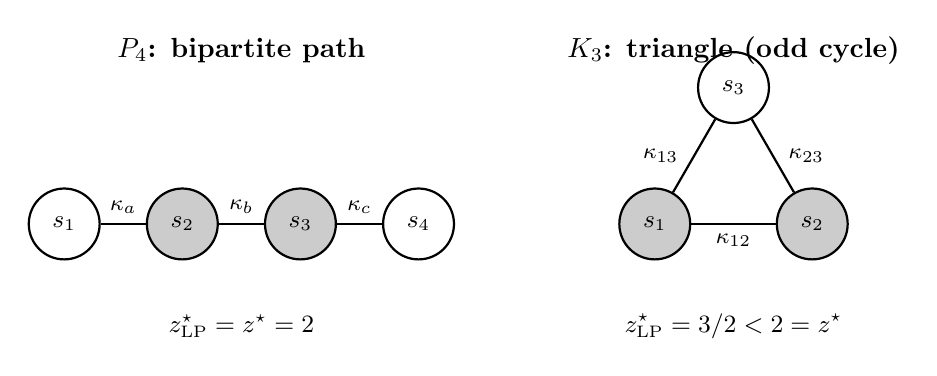
\begin{tikzpicture}[
    every node/.style={font=\small},
    vert/.style={circle, draw, thick, minimum size=9mm, inner sep=1pt},
    covered/.style={vert, fill=black!20},
    elbl/.style={font=\footnotesize},
    title/.style={font=\bfseries},
]
% Left panel: P_4
\begin{scope}
  \node[title] at (2.25,2.2) {$P_4$: bipartite path};
  \node[vert]    (a1) at (0,0)   {$s_1$};
  \node[covered] (a2) at (1.5,0) {$s_2$};
  \node[covered] (a3) at (3,0)   {$s_3$};
  \node[vert]    (a4) at (4.5,0) {$s_4$};
  \draw[thick] (a1) -- node[elbl, above] {$\kappa_a$} (a2);
  \draw[thick] (a2) -- node[elbl, above] {$\kappa_b$} (a3);
  \draw[thick] (a3) -- node[elbl, above] {$\kappa_c$} (a4);
  \node at (2.25,-1.3) {$z^\star_{\mathrm{LP}} = z^\star = 2$};
\end{scope}
% Right panel: K_3
\begin{scope}[xshift=7.5cm]
  \node[title] at (1,2.2) {$K_3$: triangle (odd cycle)};
  \node[covered] (b1) at (0,0)        {$s_1$};
  \node[covered] (b2) at (2,0)        {$s_2$};
  \node[vert]    (b3) at (1,1.732)    {$s_3$};
  \draw[thick] (b1) -- node[elbl, below]     {$\kappa_{12}$} (b2);
  \draw[thick] (b1) -- node[elbl, left=2pt]  {$\kappa_{13}$} (b3);
  \draw[thick] (b2) -- node[elbl, right=2pt] {$\kappa_{23}$} (b3);
  \node at (1,-1.3) {$z^\star_{\mathrm{LP}} = 3/2 < 2 = z^\star$};
\end{scope}
\end{tikzpicture}
\caption{The two instances as graphs whose vertices are soft clauses and
whose edges are the minimal cores. Shaded vertices give an optimal integer
hitting set $H^\star$. On the bipartite path $P_4$ (left) the LP relaxation
of the hitting-set polytope is integral, so IHS-IP, IHS-LP, and
Dantzig--Wolfe column generation all return the same value~$2$. On the
triangle $K_3$ (right) the LP optimum is $y_1 = y_2 = y_3 = \tfrac12$ with
value $3/2$, whereas any integer cover has size~$2$; the $4/3$
integrality gap is exactly where pure Dantzig--Wolfe (terminating at $3/2$)
and the integer-master IHS used in practice (returning $2$) part ways.}
\label{fig:p4-k3}
\end{figure}

\subsubsection{The Instance \texorpdfstring{$K_3$}{K3}}

Three soft unit clauses with unit weight and the ``at most one true'' hard
clauses,
\[
s_1=(x_1),\ s_2=(x_2),\ s_3=(x_3),\quad w_i=1,\qquad
\mathcal{H} = \{(\bar x_1\vee\bar x_2),\ (\bar x_1\vee\bar x_3),\ (\bar x_2\vee\bar x_3)\}.
\]
Each singleton is satisfiable; each pair is a minimal core, and the triple is
not minimal. The \textbf{minimal cores are the three pairs}
\[
\kappa_{12}=\{s_1,s_2\},\quad \kappa_{13}=\{s_1,s_3\},\quad \kappa_{23}=\{s_2,s_3\},
\]
forming a triangle $K_3$---an \emph{odd} cycle, hence non-bipartite, hence with
a fractional vertex-cover gap. For the true MaxSAT optimum, since at most one $x_i$ may be
true, at least two soft clauses must be falsified, and $z^\star = 2$.

\subsubsection{What DW Computes}
\label{sec:dwcomputes}

The full dual packing LP~\eqref{eq:pack} is
\[
\max\ \lambda_{12}+\lambda_{13}+\lambda_{23}
\quad\text{s.t.}\quad
\underbrace{\lambda_{12}+\lambda_{13}}_{s_1}\le1,\
\underbrace{\lambda_{12}+\lambda_{23}}_{s_2}\le1,\
\underbrace{\lambda_{13}+\lambda_{23}}_{s_3}\le1,\
\lambda\ge0.
\]
Summing the three constraints gives $2(\lambda_{12}+\lambda_{13}+\lambda_{23})
\le 3$, so the objective is at most $3/2$, attained at $\lambda_{12} =
\lambda_{13} = \lambda_{23} = \tfrac12$. Dually $y_1=y_2=y_3=\tfrac12$ is primal
optimal with cost $3/2$. Column generation reaches exactly this: after all three
cores are columns, the prices are $y=(\tfrac12,\tfrac12,\tfrac12)$, every core
has reduced cost $1 - (\tfrac12+\tfrac12) = 0$, no improving column exists, and
DW \textbf{terminates with value $\boldsymbol{3/2}$}. This is confirmed
empirically by the prototype \texttt{IHSSolver} in \texttt{src/ihs.py}, which
implements \cref{alg:ihs} with the master solved both as a 0/1 IP
(via PuLP/CBC) and as an LP relaxation, calling MiniSat-family assumption
SAT for the oracle. On the 3-clause WCNF encoding \texttt{src/wcnf/k3.wcnf}
the IP master returns cost $2$ (matching $z^\star$) while the LP master
value stabilizes at exactly $1.5$ (matching $z^\star_{\mathrm{LP}}$), so
both halves of \cref{tab:counter} are observed in a single run.

\subsubsection{What IHS Computes}
\label{sec:ihscomputes}

IHS generates the same three cores, but its master is the \emph{integer} hitting
set
\[
\min\ y_1+y_2+y_3 \quad\text{s.t.}\quad y_1+y_2\ge1,\ y_1+y_3\ge1,\ y_2+y_3\ge1,\ y\in\{0,1\}^3,
\]
whose optimum is $2$ (e.g.\ $H^\star=\{s_1,s_2\}$). The SAT oracle on
$\mathcal{H}\cup(\mathcal{S}\setminus H^\star)=\mathcal{H}\cup\{(x_3)\}$ succeeds
($x_3$ true, $x_1,x_2$ false), certifying a correction set of cost $2$. IHS
\textbf{terminates with value $\boldsymbol{2} = z^\star$}.

\begin{table}[htbp]
\centering
\small
\begin{tabular}{l c c c}
\toprule
& cores generated & terminal value & is it $z^\star=2$? \\
\midrule
DW / column generation on \eqref{eq:pack} & $\kappa_{12},\kappa_{13},\kappa_{23}$ & $3/2$ & \textbf{no} \\
IHS-LP (LP master) & $\kappa_{12},\kappa_{13},\kappa_{23}$ & $3/2$ & \textbf{no} \\
IHS-IP (integer master, real solvers) & $\kappa_{12},\kappa_{13},\kappa_{23}$ & $2$ & \textbf{yes} \\
\bottomrule
\end{tabular}
\caption{On the triangle $K_3$, DW and IHS-LP agree with each other (value
$3/2$) but disagree with IHS-IP and with the true optimum (value $2$). The gap
is the integrality gap $z^\star/z^\star_{\mathrm{LP}} = 4/3$ of the hitting-set
polytope.}
\label{tab:counter}
\end{table}

\begin{proposition}[Non-equivalence in general]
\label[proposition]{prop:nonequiv}
There is a MaxSAT instance on which Dantzig--Wolfe column generation on the dual
packing LP and the IHS algorithm used by practical solvers terminate with
different values. Hence practical IHS is \emph{not} equivalent to Dantzig--Wolfe
decomposition.
\end{proposition}

\begin{proof}
The triangle instance $K_3$. DW terminates at $z^\star_{\mathrm{LP}} = 3/2$
(\cref{sec:dwcomputes}); IHS-IP terminates at $z^\star = 2$
(\cref{sec:ihscomputes}). $3/2 \ne 2$.
\end{proof}

The counterexample is not pathological: $K_3$ is the smallest odd cycle, and the
same $4/3$ gap appears in every odd-cycle / fractional-cover MaxSAT instance.
\cref{tab:counter} also records the consistent reading of
\cref{prop:equiv}: IHS-\emph{LP} \emph{does} match DW (both $3/2$);
it is the \emph{integer} master that creates the discrepancy---and the integer
master is precisely what makes IHS a correct MaxSAT solver.

\paragraph{Unweighted vs weighted.} The $4/3$ figure above is the
\emph{unweighted} vertex-cover gap on $K_3$, and on this conflict graph uniform
weights are in fact extremal. For weights $w_1 \le w_2 \le w_3$ on the three
soft clauses, the integer optimum is the cheapest pair, $z^\star = w_1 + w_2$,
while half-integrality of the vertex-cover LP gives
$z^\star_{\mathrm{LP}} = \min\{\, w_1 + w_2,\ (w_1 + w_2 + w_3)/2 \,\}$. If
$w_3 \ge w_1 + w_2$, the LP optimum is integral and the gap closes entirely: the
master solution is then integral and DW coincides with IHS. Otherwise the gap
is $2(w_1+w_2)/(w_1+w_2+w_3) \in (1, 4/3]$, with the maximum exactly at
uniform weights. Weight imbalance therefore \emph{shrinks} the gap on a fixed
conflict graph---consistent with the general bound of $2$ for weighted vertex
cover. The qualitative picture (DW terminates at $z^\star_{\mathrm{LP}}$, IHS-IP
at $z^\star$) carries over verbatim to weighted instances; only the size of
the gap is instance-dependent.

%----------------------------------------------------------------------
\subsection{Reconciliation and Subtleties}
\label{sec:subtle}
%----------------------------------------------------------------------

The two results are not in tension; together they locate the equivalence
exactly.

\begin{enumerate}[label=\textbf{\arabic*.}, leftmargin=*]
\item \textbf{LP vs.\ integer master (the decisive point).}
Pure Dantzig--Wolfe is an \emph{LP} algorithm: it converges to
$z^\star_{\mathrm{LP}}$, the value of the LP relaxation, which is the
``Dantzig--Wolfe bound.'' IHS-LP shares this and is genuinely DW
(\cref{prop:equiv}). But practical IHS solves the restricted master
as an \emph{integer} program, returning $z^\star \ge z^\star_{\mathrm{LP}}$ and
closing the integrality gap. This is no longer LP column generation; it is the
combinatorial analogue of \emph{branch-and-price}. In branch-and-price,
one would branch on $y_i$ whenever the column-generation phase terminates at a
fractional $z^\star_{\mathrm{LP}}$. IHS-IP effectively performs this "branching"
implicitly and globally by solving the master as an IP at every iteration,
collapsing the entire branch-and-bound tree into a sequence of flat master
solves. The integer master is exactly what lets IHS return $2$ rather than $3/2$
on $K_3$.

\item \textbf{Pricing is separation, not optimization.}
Classical DW pricing solves an \emph{optimization}---$\min_{p\in\mathcal{P}}
(c - A^\top\pi)^\top p$---and returns the \emph{most} negative reduced-cost
column. The SAT oracle in IHS returns \emph{some} unhit core, not the
most-violated one (indeed there is no natural ``most violated'' core to ask
for). Both are correct---any improving column suffices for column-generation
convergence---but IHS uses the oracle as a \emph{separation} oracle, the flavour
of cutting planes, rather than as a reduced-cost minimizer. This is a difference
in the kind of subproblem, even where the bound agrees. Moreover, by
\cref{rem:fracpricing}, even \emph{separation} against fractional prices
exceeds a single SAT call; the plain SAT oracle implements separation only at
integral master solutions---which the integer master of practical IHS
conveniently guarantees.

\item \textbf{No convexity constraint.}
The dual packing LP~\eqref{eq:pack} has no row $\sum_\kappa \lambda_\kappa = 1$.
Strictly, then, IHS-LP is \emph{column generation}, and Dantzig--Wolfe is the
special case of column generation in which the columns are the extreme points
(and rays) of a fixed subproblem polyhedron $\mathcal{P}$ and carry a convexity
constraint. Here the ``columns'' are the cores---an implicitly defined
combinatorial family (the minimal unsatisfiable subsets), not the vertices of a
single given polyhedron. Calling this ``Dantzig--Wolfe'' rather than ``column
generation / Benders-in-the-dual'' is a mild and common abuse; it is exact only
under the dual reading of \cref{lem:rowcol}.

\item \textbf{IHS lives on the Benders$\,\leftrightarrow\,$DW bridge.}
On the primal side IHS adds \emph{rows} (cores) to a master over the
complicating variables $y$---textbook \emph{Benders / cutting planes}. By
\cref{lem:rowcol} that is identically \emph{column generation
(Dantzig--Wolfe)} on the dual. So the duality square of \cref{sec:unified}
is right: IHS is simultaneously a Benders-style and a DW-style method, the two
being the same LP object seen from opposite sides. The single caveat the square
omits is that the practical master is integer, which sits \emph{above} both LP
methods.
\end{enumerate}


%----------------------------------------------------------------------
\subsection{Verdict}
\label{sec:verdict}
%----------------------------------------------------------------------

\begin{itemize}
\item \textbf{Yes, equivalently---at the LP level.} IHS with an LP master is
\emph{exactly} Dantzig--Wolfe column generation on the dual core-packing LP:
same working set, same bound, same generated cores, same termination
(\cref{prop:equiv}). The $P_4$ trace (\cref{sec:worked}) shows this
happening step for step, and the equivalence is unconditional whenever the
hitting-set polytope is integral (e.g.\ bipartite conflict structure), where
$z^\star = z^\star_{\mathrm{LP}}$.

\item \textbf{No, not in general---because of the integer master.} The IHS used
by real solvers solves the master as an integer program and returns the true
MaxSAT optimum $z^\star$. The triangle $K_3$ (\cref{sec:counter}) is a concrete
counterexample: DW (and IHS-LP) terminate at $3/2$, while IHS-IP and the true
optimum are $2$. Practical IHS is therefore \emph{strictly stronger} than
Dantzig--Wolfe; it equals ``DW master $+$ integrality,'' i.e.\ a branch-and-price
/ integer-cutting-plane method, not pure DW.
\end{itemize}

\noindent
In one sentence: \emph{IHS is Dantzig--Wolfe on the dual packing LP precisely up
to the integrality gap of the hitting-set polytope---and that gap, which DW
cannot close but the integer IHS master can, is exactly what makes IHS a correct
MaxSAT solver rather than merely an LP-bound computation.}

%----------------------------------------------------------------------
\subsection{Closing the Gap: Pricing-Side Techniques from Column Generation}
\label{sec:cg-gap}
%----------------------------------------------------------------------

The analysis so far is diagnostic: practical IHS is column generation up to
two deviations on the pricing side. The oracle performs \emph{separation}
rather than reduced-cost \emph{optimization} (\cref{sec:subtle}, point~2),
and it separates only against \emph{integral} prices---fractional pricing
being a weighted-MUS optimization that no single SAT call implements
(\cref{rem:fracpricing}). This subsection turns the diagnosis prescriptive:
we collect three techniques that close part of the distance to genuine
column generation while keeping an \emph{unmodified} assumption-based SAT
oracle. They correspond one-for-one to three standard ingredients of
industrial column generation---approximate pricing rules, partial pricing
over a restricted column pool, and column
aggregation~\citep{desaulniers2005column}. The first two are outer-loop
schedules over ordinary SAT calls; the third already exists in the MaxSAT
literature as \emph{abstract cores}~\citep{berg2020abstract}, and the
decomposition view explains both why it works and why it is the strongest
of the three.

\subsubsection{Price-Guided Separation: Approximating the Pricing Problem}
\label{sec:price-guided}

Fix a fractional optimum $\bar y$ of the restricted master LP. Exact
pricing for the dual packing LP~\eqref{eq:pack} asks for
\begin{equation}
\pi(\bar y) \;=\; \min_{\kappa \in \mathcal{K}} \; \sum_{s_i \in \kappa} \bar y_i,
\label{eq:pricing}
\end{equation}
an improving column existing iff $\pi(\bar y) < 1$
(\cref{lem:rowcol}(ii)). Rather than solve \eqref{eq:pricing} exactly, we
bracket it with a \emph{threshold sweep}. Let $\theta_1 < \cdots < \theta_r$
enumerate the distinct values of $\bar y$ and let
$S(\theta) = \{\, s_i : \bar y_i \le \theta \,\}$ be the soft clauses whose
current dual price is at most $\theta$. Since $S(\theta) \subseteq
S(\theta')$ for $\theta \le \theta'$, unsatisfiability of $\mathcal{H} \cup
S(\theta)$ is monotone in $\theta$, so binary search with $O(\log r)$
assumption-based SAT calls finds the least infeasible level
$\theta^\dagger = \min\{\theta : \mathcal{H} \cup S(\theta) \text{ UNSAT}\}$
(when one exists), together with a core $\kappa \subseteq
S(\theta^\dagger)$.

\begin{lemma}[Price bound for the threshold sweep]
\label[lemma]{lem:sweep}
Any core $\kappa \subseteq S(\theta)$ satisfies $\sum_{s_i \in \kappa}
\bar y_i \le \theta\,|\kappa|$, so its column has reduced cost at least
$1 - \theta|\kappa|$; in particular every core found at level $\theta$ with
$|\kappa| < 1/\theta$ is an improving column for the restricted dual.
Moreover no core exists inside any $S(\theta)$ with $\theta <
\theta^\dagger$, so cores over $S(\theta^\dagger)$ are supported entirely
on the cheapest-priced clauses that support any core at all.
\end{lemma}

\begin{proof}
Each of the $|\kappa|$ terms is at most $\theta$ by membership in
$S(\theta)$; the reduced-cost statement is then \cref{lem:rowcol}(ii). The
last claim is the minimality of $\theta^\dagger$ under the monotonicity of
$S(\cdot)$.
\end{proof}

Three remarks on deployment. First, the bound $\theta|\kappa|$ rewards
\emph{core minimization}: trimming $\kappa$ to a minimal core shrinks
$|\kappa|$ and tightens the violation estimate, so the sweep and
core-trimming compose multiplicatively. Second, the sweep strictly
subsumes the price-aware assumption ordering of \cref{sec:part1}
(\cref{sec:techniques}): ordering biases the solver's conflict analysis
\emph{within} a fixed enforced set, whereas the sweep changes the enforced
set itself, and both leave CDCL internals untouched. Third, the sweep is a
\emph{heuristic} separator: a violated core mixing cheap and expensive
clauses can escape every level below its most expensive member.
Correctness is unaffected---any core it returns is a valid master
row---but termination must still be certified by the standard probe at the
integral $H^\star$, exactly as in \cref{alg:ihs}. The sweep therefore
slots in as a bound-improvement phase between master solves, never as a
replacement for the terminal check.

\subsubsection{Weight Stratification as Partial Pricing}
\label{sec:stratified}

In weighted instances the packing constraints~\eqref{eq:pack} are
heterogeneous: a core $\kappa$ can carry dual weight at most
$\min_{s_i \in \kappa} w_i$, its bottleneck capacity---this is why a
disjoint-core phase certifies the lower bound $\sum_j \min_{s_i \in
\kappa_j} w_i$. Columns supported on high-weight clauses are thus the ones
able to raise the dual objective fastest. \emph{Stratification}, introduced
for SAT-based weighted MaxSAT by \citet{ansotegui2012improving}, exploits
exactly this: partition the soft clauses into strata by descending weight,
enforce only the top stratum and extract cores until the oracle answers
SAT, then merge in the next stratum, and so on.

In column-generation terms this is \emph{partial pricing over a restricted
column pool}~\citep{desaulniers2005column}: pricing is restricted to
columns supported on the active strata---the high-capacity rows---and the
pool is enlarged only when the restricted pricing problem prices out,
which is precisely the SAT answer on the active strata. The correctness
condition transfers verbatim: optimality may be declared only when
\emph{exact} pricing over the full pool finds no improving column, i.e.,
the terminal IHS probe must enforce all soft clauses outside $H^\star$.
Everything before that terminal check is bound improvement and is free to
be restricted.

The two schedules compose naturally: within the active stratum, sweep by
dual price as in \cref{sec:price-guided}. Stratification selects the rows
with the \emph{capacity} to absorb new dual weight (primal cost $w$); the
sweep selects, among those, the rows currently \emph{underpriced} by the
master (dual price $\bar y$). This primal--dual pairing is the standard
design space of pricing rules in large-scale column generation, imported
wholesale into the IHS outer loop.

\subsubsection{Abstract Cores as Column Aggregation}
\label{sec:abstract-cores}

Large weighted instances typically contain many near-interchangeable soft
clauses, hence exponentially many near-symmetric cores: the master
accumulates rows the LP cannot tell apart, and column generation stalls.
This is a classical pathology with a classical remedy,
\emph{aggregation}: group interchangeable subproblems and replace their
individual columns by aggregate ones~\citep{desaulniers2005column}. The
MaxSAT analogue already exists: \emph{abstract
cores}~\citep{berg2020abstract}. Choose an abstraction set $A \subseteq
\mathcal{S}$ (in practice, clauses of similar weight---note the kinship
with the strata of \cref{sec:stratified}); introduce counting literals,
defined by a cardinality encoding, asserting ``at least $k$ clauses of $A$
are falsified.'' An abstract core is a core expressed over counting
literals; in the simplest case it induces the master row
\begin{equation}
\sum_{s_i \in A} y_i \;\ge\; k.
\label{eq:abstract-row}
\end{equation}
Both readings of \eqref{eq:abstract-row} are instructive.

\paragraph{Dual reading: one column for exponentially many.} In the
packing dual, \eqref{eq:abstract-row} is a single column with objective
coefficient $k$ and incidence vector $\mathbf 1_A$. Using $y_i \le 1$, it
dominates the $\binom{|A|}{|A|-k+1}$ ordinary rows $\sum_{s_i \in S} y_i
\ge 1$ for $S \subseteq A$, $|S| = |A|-k+1$ (each such $S$ is indeed a
core: if fewer than one clause of $S$ were falsified, fewer than $k$
clauses of $A$ would be). One SAT call over counting literals prices this
aggregate column; without aggregation, the same dual progress costs up to
$\binom{|A|}{|A|-k+1}$ separate core extractions over symmetric
subsets. This is column aggregation executed by a cardinality encoding.

\paragraph{Primal reading: rank-$k$ rows tighten the LP master.} Row
\eqref{eq:abstract-row} is in general \emph{not} implied by the ordinary
core rows at the LP level, so abstract cores strictly strengthen the
relaxation. The triangle of \cref{sec:counter} is the minimal witness: the
three ordinary rows $y_i + y_j \ge 1$ admit the fractional point
$(\tfrac12,\tfrac12,\tfrac12)$ of value $3/2$, whereas the abstract core
$y_1 + y_2 + y_3 \ge 2$---valid because at most one $x_i$ can be true, so
at least two soft clauses are falsified---forces value $2 = z^\star$.
Indeed on $K_3$ row~\eqref{eq:abstract-row} is precisely the
Chv\'atal--Gomory rounding of the three edge rows, the odd-cycle
inequality. Abstract cores therefore do more than aggregate: they close
part of the integrality gap that \cref{prop:nonequiv} identified as the
exact distance between pure Dantzig--Wolfe and practical IHS. In the terms
of \cref{tab:counter}, they move IHS-LP upward from $3/2$ toward $2$
without invoking the integer master.

The crux, as in DW aggregation, is choosing what to aggregate:
\citet{berg2020abstract} cluster clauses by weight similarity, and report
substantial gains inside an IHS solver on weighted benchmarks. The
decomposition view suggests a dual-informed refinement---cluster clauses
whose LP prices $\bar y_i$ move together across master iterations, i.e.,
aggregate rows the master already treats as interchangeable---which to our
knowledge is unexplored.

\paragraph{Summary.} The three techniques upgrade the IHS oracle from
``return any violated row'' toward the pricing discipline of industrial
column generation: cheap columns first (\cref{sec:price-guided}),
high-capacity columns first (\cref{sec:stratified}), and aggregated
columns where symmetry would otherwise force exponentially many
(\cref{sec:abstract-cores})---all at the outer-loop level, with CDCL
internals untouched, and with the terminal integral probe of
\cref{alg:ihs} preserved so that correctness never depends on the
heuristic pricing.

\subsubsection{An Empirical Check: How Much of the Gap Do Rank-\texorpdfstring{$k$}{k} Rows Recover?}
\label{sec:gap-empirical}

The threshold sweep (\cref{sec:price-guided}) and abstract cores
(\cref{sec:abstract-cores}) are implemented in the prototype
\texttt{IHSSolver} (\texttt{src/ihs.py}, options \texttt{threshold\_sweep}
and \texttt{auto\_abstraction}/\texttt{abstraction\_sets}); the experiment
below is reproduced by \texttt{src/gap\_benchmarks.py}. The question it
answers is the one \cref{prop:nonequiv} leaves open: on instances with a
positive integrality gap, how much of the distance $z^\star -
z^\star_{\mathrm{LP}}$ do the abstract-core rows recover in the \emph{LP
relaxation} of the master---i.e., without invoking the integer master?

\paragraph{An implementation subtlety: mixed cores are disjunctions.}
One point surfaced by the implementation deserves record, because it is
invisible in the single-set reading of \eqref{eq:abstract-row}. When the
abstract probe enforces per-set falsification \emph{counts} $t_A$ and the
oracle's core mixes counting literals of several abstraction sets, the
information returned is a \emph{disjunction}---some set $A$ in the core
must exceed its count $t_A$---not a linear row; the naive sum
$\sum_{A} \sum_{i \in A} y_i \ge 1 + \sum_A t_A$ is unsound. The exact
treatment adds an indicator per disjunct to the IP master
($\sum_{i\in A} y_i \ge (t_A{+}1)\,z_A$ with $\sum_A z_A \ge 1$), whose LP
projection is the normalized surrogate
$\sum_A \tfrac{1}{t_A+1} \sum_{i \in A} y_i \ge 1$. Only a
\emph{single-set} core yields the pure rank-$k$ row
\eqref{eq:abstract-row}. This is the LP-level face of the aggregation
trade-off: rows are strong exactly when the oracle's cores respect the
abstraction sets.

\begin{figure}[htbp]
\centering
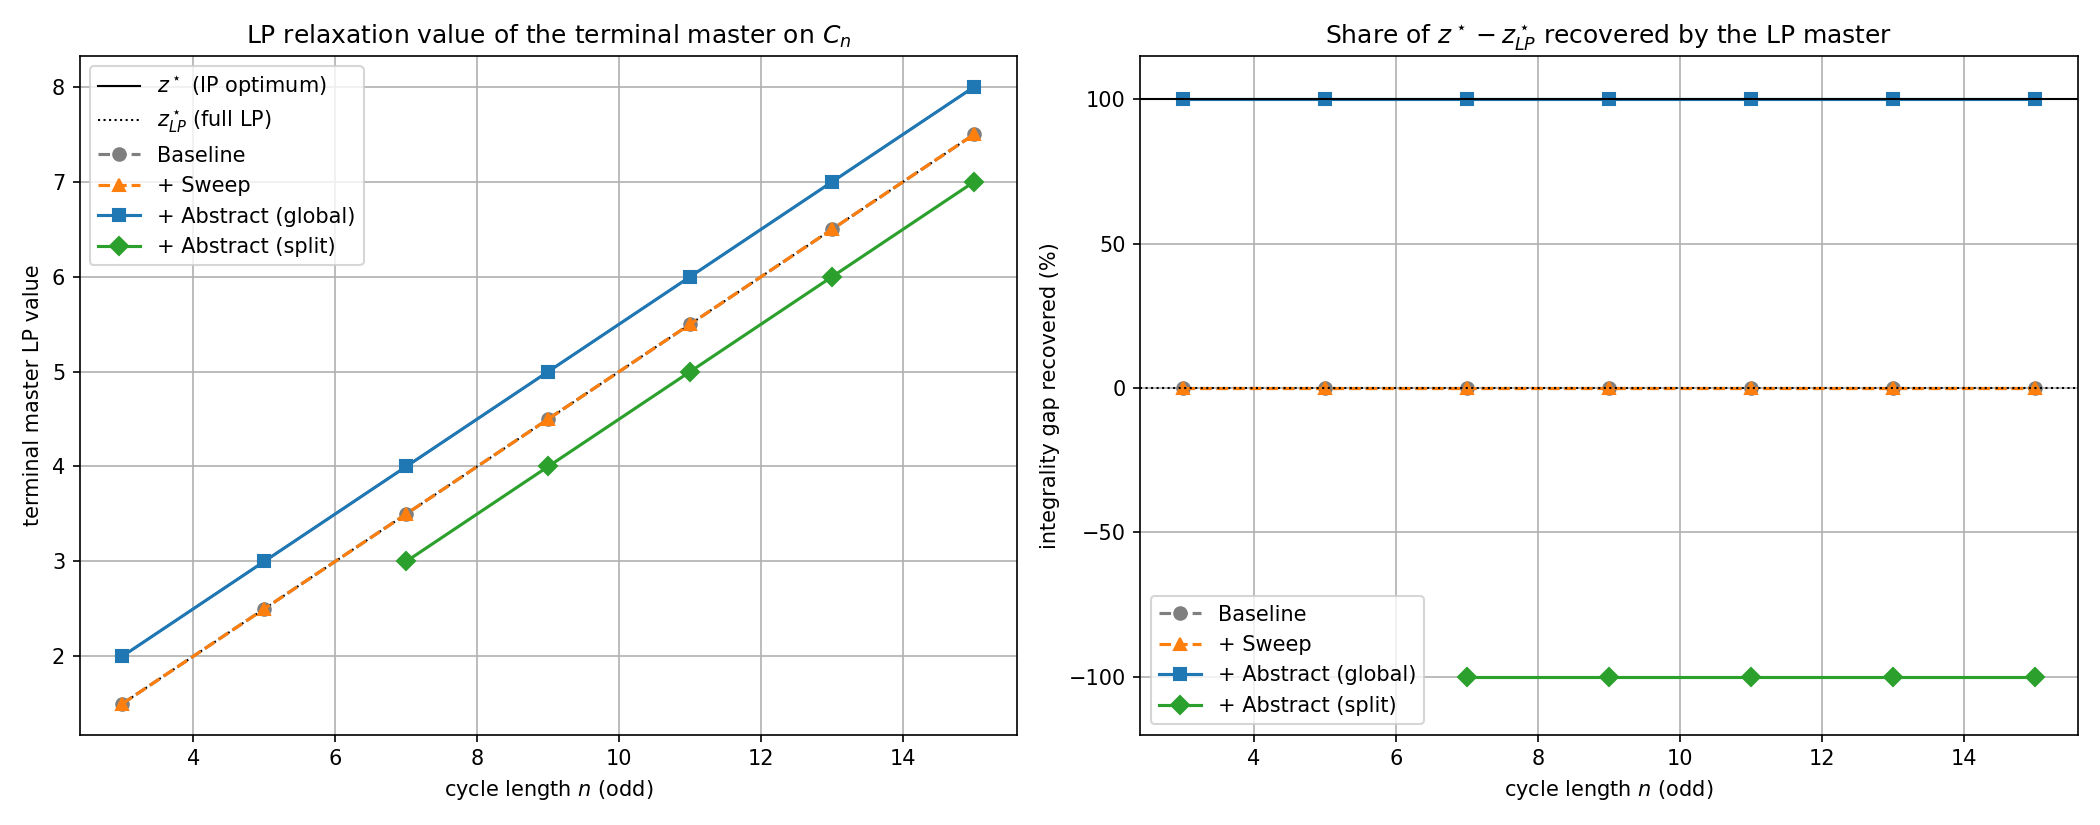
\includegraphics[width=\textwidth]{gap_plot.png}
\caption{Gap recovery on odd cycles $C_n$ (unit weights; $z^\star_{\mathrm{LP}} = n/2$,
$z^\star = (n{+}1)/2$). Left: LP relaxation value of the terminal master.
Right: share of the integrality gap recovered. One aligned abstraction set
covering the cycle recovers the \emph{entire} gap at every size; the split
two-arc clustering produces only mixed (disjunctive) cores and recovers
nothing; the threshold sweep coincides with the baseline because uniform
prices $\bar y_i = \tfrac12$ collapse the sweep to the standard probe.}
\label{fig:gap_recovery}
\end{figure}

\paragraph{Odd cycles: full recovery under aligned aggregation.}
\Cref{fig:gap_recovery} generalizes the $K_3$ counterexample to odd cycles
$C_n$, the canonical family with a persistent vertex-cover gap of
$\tfrac12$. With a single abstraction set covering the cycle, the terminal
LP master attains $z^\star$ at every size---the odd-cycle inequality of
\cref{sec:abstract-cores}, discovered automatically as a rank-$k$
row---while the outer loop shortens from $n{+}1$ iterations (the baseline
must enumerate all $n$ edge cores) to $(n{+}3)/2$. Splitting the same
clauses into two contiguous arcs destroys both effects: every core now
straddles the two sets, only weak normalized surrogates enter the LP, and
the terminal LP value drops \emph{below} $z^\star_{\mathrm{LP}}$ (the run
terminates before accumulating the edge rows the baseline collects).

\paragraph{The aggregation limit is core-guided search.} With one
uniform-weight set covering all soft clauses, the abstract probe asks
``is there a solution falsifying at most $t$ clauses?'' and increments
$t$ on each UNSAT answer---that is, IHS at full aggregation \emph{is} a
core-guided-style linear search over a single cardinality bound (cf.\ the
MSU family of \cref{sec:part1}). The aggregation axis thus interpolates
between the two algorithm families of the duality square
(\cref{sec:unified}): no aggregation is pure IHS, full aggregation is
linear-search core-guided, and the useful regime of abstract cores lies
strictly between.

\begin{table}[htbp]
\centering
\small
\caption{Aggregation alignment on random vertex cover $G(n, 0.2)$
(means over three seeds; CBC/MiniSat prototype). Unit weights give
one aligned global abstraction set; weights drawn from $\{1,2,3\}$ give
three weight-class clusters that cut across the conflict structure.
``Gap rec.''\ is the share of $z^\star - z^\star_{\mathrm{LP}}$ recovered
by the terminal LP master (negative when the terminal master is weaker
than the full ordinary-row LP).}
\label{tab:alignment}
\begin{tabular}{llrrrr}
\toprule
\textbf{Family} & \textbf{Config.} & \textbf{Gap rec.} & \textbf{Iter.} & \textbf{SAT} & \textbf{Time} \\
\midrule
unit, $n{=}25$     & Baseline  & $-7\%$   & $43.0$  & $43.0$  & $1.3$s \\
                   & + Sweep   & $0\%$    & $41.0$  & $89.0$  & $1.3$s \\
                   & + Abstract& $100\%$  & $15.3$  & $15.3$  & $0.4$s \\
\midrule
unit, $n{=}35$     & Baseline  & $0\%$    & $102.0$ & $102.0$ & $3.8$s \\
                   & + Sweep   & $0\%$    & $92.7$  & $202.3$ & $3.5$s \\
                   & + Abstract& $100\%$  & $23.7$  & $23.7$  & $0.7$s \\
\midrule
weighted, $n{=}25$ & Baseline  & $-56\%$  & $43.3$  & $43.3$  & $1.3$s \\
                   & + Sweep   & $-33\%$  & $38.3$  & $81.7$  & $1.2$s \\
                   & + Abstract& $-198\%$ & $40.0$  & $71.7$  & $8.0$s \\
\midrule
weighted, $n{=}35$ & Baseline  & $-2\%$   & $87.7$  & $87.7$  & $3.4$s \\
                   & + Sweep   & $-2\%$   & $82.7$  & $193.3$ & $3.2$s \\
                   & + Abstract& $-1\%$   & $99.0$  & $185.0$ & $36.9$s \\
\bottomrule
\end{tabular}
\end{table}

\paragraph{Random vertex cover: alignment decides the sign of the effect.}
\Cref{tab:alignment} repeats the comparison on random $G(n, 0.2)$ vertex
cover, where the gap arises from many overlapping odd structures rather
than one cycle. Under aligned aggregation (unit weights, one global set)
abstract cores again recover $100\%$ of the gap while cutting iterations
by $3$--$4\times$ and wall time by $5\times$. Under misaligned aggregation
(three weight-class clusters) the effect \emph{reverses}: nearly all cores
are mixed, the LP master gains nothing, SAT calls double, and the
indicator-laden IP master becomes markedly heavier. All configurations
return $z^\star$ in all runs---correctness never depends on the
aggregation---but the profitable regime is exactly the aligned one. This
is the measured face of the crux noted in \cref{sec:abstract-cores}
(``choosing what to aggregate'') and sharpens the motivation for the
dual-informed clustering proposed there: clusters should follow the
conflict structure the master actually prices, not the weight profile
alone. The threshold sweep, for its part, behaves as billed: inert under
uniform prices (odd cycles), and a cheap bound-improvement phase under
heterogeneous prices ($6$--$12\%$ fewer iterations at roughly twice the
SAT calls, time-neutral at prototype scale).


%======================================================================
\part*{Part III — Empirical Evaluation of IHS for Weighted CSPs (Petrova, Larrosa, Roll\'on, 2025)}
\addcontentsline{toc}{part}{Part III — Empirical Evaluation of IHS for Weighted CSPs}
%======================================================================

\begin{abstract}
This part summarizes the method and findings of~\citet{petrova2025empirical},
who carry out an empirical study of IHS for the Weighted CSP framework. Where
Parts~I--II frame IHS theoretically as Dantzig--Wolfe on the dual packing LP,
Petrova et~al.\ vary the two main algorithmic axes (computation of hitting
vectors and core improvement) and report on 32 configurations across a
heterogeneous benchmark suite. The two studies are complementary: the OR
framing in Parts~I--II predicts that techniques relaxing the hitting-vector
subproblem and that strengthen cores should both pay off; the empirical study
confirms this is benchmark-dependent but identifies cost-function merging
combined with maximal-core extraction as the most robust default.
\end{abstract}

%----------------------------------------------------------------------
\section{Problem setting: Weighted CSP}
\label{sec:wcsp}
%----------------------------------------------------------------------

A \emph{Weighted Constraint Satisfaction Problem} (WCSP) is a triple
$(X, C, F)$ where $X$ is a set of variables over finite domains, $C$ is a set
of hard constraints (Boolean functions over scopes of $X$), and
$F = \{f_1, \ldots, f_m\}$ is a set of \emph{cost functions}, each mapping
assignments of its scope to a nonnegative cost. A solution is a complete
assignment satisfying all constraints; its cost is the sum of cost-function
values; the goal is a minimum-cost solution $w^\star$. WCSP generalizes
weighted MaxSAT: each soft clause becomes a unary cost function over its
falsification indicator, and hard clauses move into $C$.

%----------------------------------------------------------------------
\section{Vector-valued IHS for WCSP}
\label{sec:vecihs}
%----------------------------------------------------------------------

To handle multi-valued cost functions cleanly the paper recasts IHS in
vector-valued language. A \emph{cost vector}
$\vec{v} = (v_1, \ldots, v_m)$ assigns to each cost function $f_i$ a value
$v_i$ that must be an actual cost occurring in $f_i$. The vector induces a
CSP $(X, C \cup F_{\vec{v}})$ in which each soft cost function $f_i$ is
replaced by the constraint $f_i \le v_i$. If this CSP is satisfiable, $\vec{v}$
is a \emph{solution vector}; otherwise it is a \emph{core}. Costs and
dominance lift componentwise: $\vec{u} \le \vec{v}$ holds iff $u_i \le v_i$ for
all $i$; a set of vectors $\mathcal{V}$ \emph{dominates} a vector $\vec{u}$
if some $\vec{v} \in \mathcal{V}$ has $\vec{v} \le \vec{u}$. A vector that is
not dominated by a set of cores $\mathcal{K}$ is said to \emph{hit}
$\mathcal{K}$; the \emph{minimum-cost hitting vector} (MHV) of $\mathcal{K}$ is
a hitting vector of minimum cost. Computing MHV is NP-hard (it reduces to
minimum hitting set), so it is the analog of the IHS master.

Two structural bounds drive the algorithm. For any solution vector $\vec{h}$
and any set of cores $\mathcal{K} \subseteq \mathit{Cores}$,
\[
\mathit{MHV}(\mathcal{K}) \;\le\; w^\star \;\le\; \mathit{cost}(\vec{h}).
\]
The algorithm terminates when these two bounds meet. Termination is
characterized in terms of \emph{goal cores}: $\mathit{MHV}(\mathcal{K}) = w^\star$
iff $\mathcal{K}$ dominates every \emph{maximal core of cost less than
$w^\star$}. The IHS task is therefore to compute a set $\mathcal{K}$ that
dominates every such goal core and an optimal solution.

%----------------------------------------------------------------------
\section{Baseline algorithm}
\label{sec:baseline}
%----------------------------------------------------------------------

The baseline IHS algorithm (\textsc{IHS-lb}) is given in
Algorithm~\ref{alg:ihs-lb}. It maintains a working core set $\mathcal{K}$ with
a lower bound $\mathit{lb}$ and an upper bound $\mathit{ub}$. At each
iteration it computes an MHV $\vec{h}$ of $\mathcal{K}$ (raising
$\mathit{lb}$), solves the induced CSP and, if unsatisfiable, calls a routine
$\textsc{ImprCore}$ that grows $\vec{h}$ into an improved core
$\vec{k} \ge \vec{h}$, which is added to $\mathcal{K}$.

\begin{algorithm}[t]
\caption{Baseline IHS for WCSP (\textsc{IHS-lb}). $\textsc{MinCostHV}(\mathcal{K})$ returns a minimum-cost hitting vector; $\textsc{ImprCore}$ improves a hitting vector that is a core into a larger core.}
\label{alg:ihs-lb}
\begin{algorithmic}[1]
\Require WCSP $(X, C, F)$
\Ensure cost $w^\star$ of an optimal solution vector
\State $\mathcal{K} \gets \emptyset$;\ $\mathit{lb} \gets 0$;\ $\mathit{ub} \gets \infty$
\While{$\mathit{lb} < \mathit{ub}$}
  \State $\vec{h} \gets \textsc{MinCostHV}(\mathcal{K})$;\quad $\mathit{lb} \gets \mathit{cost}(\vec{h})$
  \If{$\textsc{SolveCSP}(X,\, C \cup F_{\vec{h}})$}
      \State $\mathit{ub} \gets \mathit{cost}(\vec{h})$
  \Else
      \State $\vec{k} \gets \textsc{ImprCore}(X, C, F, \mathit{ub}, \vec{h})$;\quad $\mathcal{K} \gets \mathcal{K} \cup \{\vec{k}\}$
  \EndIf
\EndWhile
\State \Return $\mathit{lb}$
\end{algorithmic}
\end{algorithm}

A symmetric variant \textsc{IHS-ub} computes a \emph{cost-bounded} hitting
vector (any hitting vector of cost less than the current $\mathit{ub}$,
solved as a decision problem) instead of the cost-minimal one, prioritizing
upper-bound tightening over lower-bound tightening. Each iteration of either
variant decomposes into two NP-hard pieces: the hitting-vector subproblem
(integer optimization) and the induced CSP (decision).

%----------------------------------------------------------------------
\section{Algorithmic alternatives (the 32 implementations)}
\label{sec:alts}
%----------------------------------------------------------------------

The paper isolates two design axes and crosses them with one preprocessing
choice, yielding $4 \times 4 \times 2 = 32$ implementations.

\subsection{Axis 1 --- Computation of hitting vectors (4 options)}

\begin{itemize}
\item \textbf{\textsc{MinCostHV} (IHS-\emph{lb}).} Optimal hitting vector via
0/1 integer programming. Each iteration strictly tightens the lower bound;
expensive per iteration.

\item \textbf{\textsc{CostBoundedHV} (IHS-\emph{ub}).} Any hitting vector of
cost less than the current $\mathit{ub}$. A decision problem, hence cheaper;
but the cost is not guaranteed to be below $w^\star$, so new cores need not
contribute to the lower bound (cf.\ the goal-cores characterization above).

\item \textbf{Greedy variant in \emph{lb} mode (IHS-\emph{grdlb}).} An
inexact, heuristic hitting-vector computation that starts from
$\vec{h} = \vec{0}$ and increments components by a ratio criterion (analogous
to greedy vertex cover). When a greedy step fails to make progress the next
iteration falls back to \textsc{MinCostHV}, preserving correctness.

\item \textbf{Greedy variant in \emph{ub} mode (IHS-\emph{grdub}).} As above,
but with fallback to \textsc{CostBoundedHV}.
\end{itemize}

The intent of relaxing \textsc{MinCostHV} to a cost-bounded or greedy variant
is the same that motivates in-out separation and dual stabilization in
column generation (Part~I, \S\ref{sec:techniques}): cheaper, less-optimal
probe points trade per-iteration cost for iteration count.

\subsection{Axis 2 --- Core improvement (\textsc{ImprCore}, 4 options)}

All four variants take a hitting vector $\vec{h}$ that is a core and grow it
into a larger core $\vec{k} \ge \vec{h}$ by incrementing components while
preserving the core condition.

\begin{itemize}
\item \textbf{Maximal cores.} Strongest and most expensive: keep incrementing
until no further component can be increased without breaking the core
condition. Analogous to destructive MUS extraction. Produces cores that
dominate the largest set of goal cores per call.

\item \textbf{Lazy cores.} Weakest and cheapest: no explicit improvement. The
assumption-based SAT solver already returns a core that is implicitly
improved at no extra cost.

\item \textbf{Cost-bounded cores.} Intermediate: improve $\vec{h}$ until its
cost reaches $\mathit{ub}$. If $\mathit{ub} > w^\star$, the resulting core
contributes to dominating goal cores; otherwise the improvement is wasted.

\item \textbf{Partially maximal cores.} Soften maximality to require only that
the increment of \emph{some} single component produces a solution vector
(rather than every component). Used in earlier work~\citep{moreno2013implicit}.
\end{itemize}

Across all four variants the implementation prefers, at each candidate step,
the component with the lowest value~$v_i$: having $\mathcal{K}$ cores whose
minimum value is as large as possible makes them more costly to hit,
accelerating the lower bound.

The maximal-cores option is the analog of Pareto-optimal core selection in
Part~I (\S\ref{sec:techniques}, \citet{magnanti1981accelerating}): both
strengthen the cuts/columns generated per oracle call at a higher
per-iteration price.

\subsection{Axis 3 --- Cost-function merging (with vs.\ without)}

A preprocessing step (see~\citet{petrova2025empirical} and references therein)
heuristically clusters cost functions along a tree decomposition and
``virtually'' merges each cluster into a single cost function with extended
domain. This shrinks the dimensionality of the cost-vector space and is shown
empirically to be the single most impactful design choice.

\subsection{Implementation choices}

\begin{itemize}
\item \textsc{MinCostHV} and \textsc{CostBoundedHV} are modelled as 0/1 IPs
and solved with \emph{CPLEX}.
\item Induced CSPs are encoded as CNF and solved with the assumption-based
SAT solver \emph{CaDiCaL}; this is what makes ``lazy cores'' free.
\item All instances are pre-processed and made \emph{virtually arc consistent}
(VAC) before solving.
\item Some iterations are allowed to extract \emph{disjunctive cores} (cores
covering multiple branches simultaneously), as in~\citet{allouche2015anytime}.
\item Time limit: 1 hour per instance.
\end{itemize}

%----------------------------------------------------------------------
\section{Empirical landscape (high-level)}
\label{sec:wcspresults}
%----------------------------------------------------------------------

The benchmark suite (12 classes) spans uniform random, scale-free random, and
structured problems (EHI, SPOT5, driverlog, Grid, Normalized, Pedigree,
CELAR), with up to a few thousand variables and cost functions per instance.

\paragraph{Cost-function merging is dominant.} Speed-ups range from $1.3\times$
(Normalized) to $268\times$ (random domains) with only the Grid class harmed
by merging---suggesting the tree-decomposition heuristic is unsuited to
its regular structure.

\paragraph{No algorithm uniformly dominates.} Different benchmark classes
prefer dramatically different combinations, with ratios up to several orders
of magnitude between the best and the worst configuration on the same
benchmark. The authors warn against concluding that IHS ``is not suitable''
for any particular benchmark class without trying multiple combinations.

\paragraph{Maximal cores are the most common best option.} For $10$ of $12$
benchmark classes maximal cores produce the best running time. Pedigree and
random-domains are the exceptions: there the induced CSPs are SAT-hard
enough that the cheaper lazy cores pay off.

\paragraph{The intermediate options are never the best for core improvement.}
Cost-bounded cores turn out to be empirically close to lazy cores (the
assumption-based SAT solver already provides cores whose cost reaches
$\mathit{ub}$); partially maximal cores tend to be too weak. Only the two
extremes (maximal or lazy) ever win.

\paragraph{Greedy hitting vectors rarely pay off.} Except in the very early
iterations, greedy variants produce cheap-but-useless iterations and end up
converging to their exact counterpart; better heuristics could plausibly
change this picture.

\paragraph{Competitiveness with the state-of-the-art.} Compared with
Toulbar2 (the leading WCSP solver), IHS still trails on most random
benchmarks but is competitive---and outperforms Toulbar2---on benchmarks with
small domains and few distinct costs (EHI, SPOT5, Grid, Normalized,
Pedigree). These two structural features (small domains, few distinct
costs) appear to be the most reliable proxy for IHS suitability.

%----------------------------------------------------------------------
\section{Connection to Parts~I and~II}
\label{sec:wcspconnect}
%----------------------------------------------------------------------

The two design axes Petrova et~al.\ vary line up cleanly with the OR-derived
techniques framed in Part~I (\S\ref{sec:techniques}).

\begin{itemize}
\item \textbf{Axis 1 (hitting-vector relaxation) $\leftrightarrow$
in-out separation / cost-bounded probing.} The paper's \textsc{CostBoundedHV}
and greedy options are concrete realizations of the idea that the master
need not be solved to optimality at every iteration; the same observation
underlies in-out separation in column generation~\citep{benameur2007stabilization}.

\item \textbf{Axis 2 (core improvement) $\leftrightarrow$ Pareto-optimal
core selection.} The maximal-cores option of Petrova et~al.\ is the
non-fractional analog of the Magnanti--Wong dominance criterion: both
strengthen the cuts/columns produced per oracle call.

\item \textbf{Axis 3 (cost-function merging) $\leftrightarrow$ Dantzig--Wolfe
preprocessing.} Tree-decomposition-based merging compresses the
constraint structure before the IHS loop, in the spirit of OR
preprocessing techniques (e.g.\ aggregation in column generation) that
reduce master dimension prior to solving.
\end{itemize}

Two features of the paper depart from the Parts~I--II framing. First, the
paper does not consider an \emph{LP-relaxation} view of the hitting-vector
subproblem, hence none of its variants exploit fractional dual prices
$\bar{y}$; the price-aware extraction and Wentges stabilization techniques
of Part~I are therefore complementary rather than overlapping. Second, the
paper does \emph{not} consider warm-starting from a complementary algorithm
(e.g.\ Toulbar2's incremental lower bound, or a short core-guided phase);
cross-family warm-starting (Part~I, \S\ref{sec:techniques}) is an
unexplored direction.

The empirical evidence on the cost-function merging axis is also a
cautionary note for theoretical analyses that treat the cost-function
collection as fixed: merging changes the effective dimensionality of the
hitting-vector space, which Parts~I--II do not model and which dominates
solver performance.

\paragraph{Summary.} Parts~I--II provide a structural reason to expect that
relaxed hitting-vector subproblems and stronger cores both help; the empirical
study of~\citet{petrova2025empirical} confirms the latter (maximal cores) and
qualifies the former (cost-bounded helps mainly via assumption-based SAT,
greedy heuristics need better design). The complementarity is clean: the OR
framing identifies the design axes worth varying, and the empirical study
populates them with measured trade-offs.




%======================================================================
\section{Closing Synthesis}
\label{sec:closing}
%======================================================================

Three observations summarize the memo.

\paragraph{The structural mapping is sound but conditional.} The pairings
core-guided $\leftrightarrow$ LBBD and IHS $\leftrightarrow$ Dantzig--Wolfe
developed in \cref{sec:part1} are correct at the level of LP duality between
primal cuts and dual columns and at the level of oracle soundness. They
break at the level of complexity (pricing is NP-complete, not polynomial),
master tractability (the practical master is integer), and primal geometry
(cores are not extreme points of a fixed polytope). Techniques whose
correctness depends only on the row--column duality should transfer;
techniques that rely on polynomial pricing or on LP master geometry should
not be expected to transfer without adaptation.

\paragraph{The integer master is exactly where IHS leaves Dantzig--Wolfe
behind.} \Cref{sec:part2} makes this precise: IHS with an LP master is
literally column generation on the dual packing LP, while the IHS used by
real solvers solves the master as an integer program and is strictly
stronger. The difference is the integrality gap of the hitting-set
polytope---vanishing on bipartite-conflict instances (the $P_4$ trace),
positive on odd-cycle instances (the $K_3$ counterexample, where DW
terminates at $3/2$ and IHS at the true optimum $2$).

\paragraph{Empirics confirm the qualitative predictions but reorder
priorities.} \Citet{petrova2025empirical}, surveyed in \cref{sec:part3},
find that stronger cores (maximal extraction)---the analog of
Pareto-optimal cut selection---pay off broadly: maximal cores are the
best option on $10$ of $12$ benchmark classes. Relaxed hitting-vector
subproblems (greedy and cost-bounded variants) pay off less than the OR
analogy alone would predict, and only at the extremes. Cost-function
merging, a preprocessing axis the framing of \cref{sec:part1,sec:part2}
does not model, is the single most impactful design choice.

\paragraph{Open directions.} Three concrete avenues stand out. (i) The
weighted case of the equivalence: the cleanest LP encodings of core-guided
algorithms~\citep{katsirelos2023analysis} cover only unweighted instances,
and the weighted analysis is open. (ii) An LP-relaxation view of the WCSP
hitting-vector subproblem would unlock the dual-stabilization and
price-aware techniques of \cref{sec:techniques} for the empirical setting
of \cref{sec:part3}. (iii) Further hybrid refinements: while basic
cross-family warm-starting is shown here to be highly effective, more
sophisticated interleaving---e.g., dynamic switching between core-guided
and IHS phases based on progress metrics---remains unexplored.

\begin{table}[h]
\centering
\caption{Empirical performance of §\ref{sec:techniques} techniques on the provided benchmarks. Iteration counts include the initial master solve. Warm-starting uses a 5-iteration Fu--Malik seed.}
\label{tab:results}
\begin{tabular}{l ccc ccc}
\toprule
& \multicolumn{3}{c}{\textbf{Weighted Chain}} & \multicolumn{3}{c}{\textbf{Triangle ($K_3$)}} \\
\cmidrule(lr){2-4} \cmidrule(lr){5-7}
\textbf{Configuration} & Cost & LP & Iters & Cost & LP & Iters \\
\midrule
Plain IHS (baseline) & 13 & 13.0 & 7 & 2 & 1.5 & 4 \\
+ Warm-start (seed)  & 13 & 13.0 & 2 & 2 & 1.5 & 2 \\
+ Hybrid (all)       & 13 & 13.0 & 2 & 2 & 1.5 & 2 \\
\bottomrule
\end{tabular}
\end{table}

\bibliographystyle{plainnat}
\bibliography{refs}

\end{document}
